% \documentclass[12pt]{article}
\documentclass[12pt]{amsart}

\pagestyle{plain}
\usepackage[margin=3cm]{geometry} 

\usepackage{amsmath,amssymb,amsfonts,enumerate,latexsym, amsthm,textcomp,wasysym,longtable}
\usepackage{mathrsfs, mathtools}
\usepackage{array,ragged2e,longtable,multirow}

% \usepackage{indentfirst}
\usepackage[matrix, arrow, curve]{xy} % Для коммутативных диаграмм
\usepackage{xy, xypic, multicol}

\usepackage[utf8]{inputenc}
\usepackage[english]{babel}
\usepackage{verbatim}
\makeatletter
\def\@settitle{\begin{center}%
		\baselineskip14\p@\relax
		\bfseries
		\large \@title
	\end{center}%
}
\makeatother

\usepackage{cancel}
\usepackage{graphicx}
% \graphicspath{{pictures/}}
% \DeclareGraphicsExtensions{.pdf,.png,.jpg}
%\usepackage{russian}

%%%%%%%%%%%%%%%%%%%%%%%%%%%%%%%%%%%%%%%%%%%%%%%%%%%%%%%%%%%%
% % commands for making comments
\usepackage[dvipsnames]{xcolor}
\newcommand{\YP}[1]{\footnote{\textcolor{red}{YP: #1}}}
\newcommand{\yp}[1]{\leavevmode{\color{red}{#1}}}
% {\textcolor{orange}{#1}} 
\usepackage[normalem]{ulem}
%%%%%%%%%%%%%%%%%%%%%%%%%%%%%%%%%%%%%%%%%%%%%%%%%%%%%%%%%%%%

\usepackage{hyperref}
\usepackage{tikz-cd} % Ещё для коммутативных диаграмм
\usetikzlibrary{babel}

% named conditions inside definitions:
% \condlabel{Z}{cond:Z} prints (Z) and sets an anchor,
% \condref{cond:Z} prints (Z) as a hyperlink
\makeatletter
\newcommand{\condlabel}[2]{\phantomsection\def\@currentlabel{#1}\label{#2}\textup{(#1)}}
\makeatother
\newcommand{\condref}[1]{\textup{(\ref{#1})}}

% \textheight=270mm
% \textwidth=190mm
% \voffset=-40mm
% \hoffset=-35mm
% \pagestyle{empty}
% 
% \\SLoppy



\newtheorem{theorem}{Theorem}
\newtheorem{proposition}[theorem]{Proposition}
\newtheorem{lemma}[theorem]{Lemma}
\newtheorem{corollary}[theorem]{Corollary}
\newenvironment{remark}{{\textbf{Remark.}}}

\numberwithin{theorem}{section}

\theoremstyle{definition}

\newtheorem{example}[theorem]{Example}

% preamble
\usepackage{etoolbox}
\AtEndEnvironment{example}{\hfill$\bigstar$}
\newcounter{pstep}
\AtBeginEnvironment{proof}{\setcounter{pstep}{0}}
\newcommand{\step}[1]{\par\medskip\noindent\refstepcounter{pstep}\textbf{Step \thepstep}\ (\textit{#1}).\ \ignorespaces}
% illustrations inside proofs: small font, slightly indented, so that they are
% visibly separate from the text of the proof
\newenvironment{illustration}{\par\medskip\begingroup\footnotesize\noindent\leftskip=1.5em\rightskip=1.5em}{\par\endgroup\medskip\noindent\ignorespaces}

%\newcommand{\defin}[2]{\hypertarget{#2}{{\color{red} #1}} \label{def:#2}}
\newcommand{\defin}[2]{\hypertarget{#2}{{\color{red} #1}}}

% Цвета
\definecolor{linkcolor}{HTML}{0000FF} % цвет ссылок
\definecolor{urlcolor}{HTML}{0000FF} % цвет гиперссылок
\definecolor{citecolor}{HTML}{0000FF} % цвет ссылки на статью
\hypersetup{pdfstartview=FitH, linkcolor=linkcolor, urlcolor=urlcolor, citecolor=citecolor, colorlinks=true}

\definecolor{completed}{HTML}{32CD32}
\definecolor{inprocessing}{HTML}{D19A0F}
\newcommand{\TODO}[1]{\textcolor{red}{НУЖНО: #1}}

\newcommand{\Alt}{\mathfrak{A}}
\newcommand{\Sym}{\mathfrak{S}}
\newcommand{\D}{\mathrm{D}}
\newcommand{\Q}{\mathrm{Q}}
\newcommand{\cyclic}{\mathrm{C}}
\newcommand{\Tetr}{\mathrm{T}}
\newcommand{\Oct}{\mathrm{O}}
\newcommand{\Ico}{\mathrm{I}}
\newcommand{\CC}{\mathbb{C}}
\newcommand{\RR}{\mathbb{R}}
\newcommand{\FF}{\mathbb{F}}
\newcommand{\EE}{\mathbb{E}}
\newcommand{\ZZ}{\mathbb{Z}}
\newcommand{\QQ}{\mathbb{Q}}
\newcommand{\HH}{\mathbb{H}}

\newcommand{\calA}{\mathcal{A}}
\newcommand{\calB}{\mathcal{B}}
\newcommand{\calE}{\mathcal{E}}
\newcommand{\calC}{\mathcal{C}}
\newcommand{\calP}{\mathcal{P}}
\newcommand{\sheafF}{\mathscr{F}}
\newcommand{\sheafG}{\mathcal{G}}

\newcommand{\GL}{\operatorname{GL}}
\newcommand{\SL}{\operatorname{SL}}
\newcommand{\PGL}{\operatorname{PGL}}
\newcommand{\PSL}{\operatorname{PSL}}
\newcommand{\SU}{\operatorname{SU}}
\newcommand{\SO}{\operatorname{SO}}
\newcommand{\diag}{\operatorname{diag}}
\newcommand{\characteristic}{\operatorname{char}}
\newcommand{\kk}{\Bbbk}

\newcommand{\pt}{\mathrm{pt}}
\newcommand{\Hom}{\mathrm{Hom}}
\newcommand{\projective}{\mathbb{P}}
\newcommand{\Id}{\mathrm{Id}}
\newcommand{\image}{\mathrm{Im} \,}
\newcommand{\aut}{\mathrm{Aut}}
\newcommand{\pr}{\operatorname{pr}}
\newcommand{\rad}{\operatorname{Rad}}
\newcommand{\ann}[1]{\operatorname{Ann}}
\newcommand{\op}{{\mathrm{op}}}
\newcommand{\End}{\operatorname{End}}
\newcommand{\Ab}{\mathrm{Ab}}
\newcommand{\grad}{\operatorname{grad}}
\newcommand{\proj}{\operatorname{Proj}}
\newcommand{\spec}{\operatorname{Spec}}
\newcommand{\gal}{\operatorname{Gal}}
\newcommand{\id}{\mathrm{Id}}
\newcommand{\tr}{\operatorname{tr}}
\newcommand{\oo}{\mathscr{O}}
\newcommand{\vect}[1]{\overrightarrow{#1}}
\newcommand{\arithmgen}{\operatorname{p}_a}
\newcommand{\geomgen}{\operatorname{p}_g}
\newcommand{\Div}{\operatorname{Div}}
\newcommand{\pic}{\operatorname{Pic}}
\newcommand{\canclass}{K}
\newcommand{\irreg}{\mathrm{q}}
\newcommand{\euler}{\chi}
\newcommand{\tangent}{\mathscr{T}}
\newcommand{\curvegen}{\operatorname{g}}
\newcommand{\basepoints}{\operatorname{Bs}}
\newcommand{\ruled}{\mathbb{F}}
\newcommand{\exc}{\operatorname{Exc}}
\newcommand{\num}{\operatorname{Num}}
\newcommand{\Ext}{\operatorname{Ext}}
\newcommand{\Kgroup}{K_0}
\newcommand{\calD}{\mathcal{D}}
\newcommand{\Dle}[1]{\calD^{\leqslant #1}}
\newcommand{\Dge}[1]{\calD^{\geqslant #1}}
\newcommand{\Cone}{\operatorname{Cone}}
\newcommand{\re}{\operatorname{Re}}
\newcommand{\im}{\operatorname{Im}}

\newcommand{\aaa}{\mathfrak{a}}
\newcommand{\bb}{\mathfrak{b}}
\newcommand{\cc}{\mathfrak{c}}
\newcommand{\pp}{\mathfrak{p}}
\newcommand{\qq}{\mathfrak{q}}
\newcommand{\mm}{\mathfrak{m}}

% Определение множества
\newcommand{\defineset}[2]{\left\{
	\left.
	#1
	\right\vert
	#2
	\right\}}

\newcommand{\spmatrix}[4]{
	\left( \begin{smallmatrix}
		#1 & #2 \\
		#3 & #4
	\end{smallmatrix} \right)
}


% Кусочное определение функции
\newcommand{\definefuntwo}[4]{
	\begin{cases}
		#1, & #2; \\
		#3, & #4.
	\end{cases}
}

\newcommand{\definefunthree}[6]{
	\begin{cases}
		#1, & #2; \\
		#3, & #4; \\
		#5, & #6.
	\end{cases}
}

\newcommand{\definefunfour}[8]{
	\begin{cases}
		#1, & #2; \\
		#3, & #4; \\
		#5, & #6; \\
		#7, & #8.
	\end{cases}
}


\newcommand{\red}[1]{{\color{red} #1}}
\newcommand{\blue}[1]{{\color{blue} #1}}


\renewcommand\labelenumi{\rm (\arabic{enumi})}
\renewcommand\theenumi{\rm (\arabic{enumi})}

\newcolumntype{C}[1]{%
	>{\vspace{0pt}\Centering\arraybackslash}m{#1}%
}


\newcommand{\groupinfo}[5]{
	#1 & #2 & #3 & #4 & #5 \\
}


\title{Bridgeland Stability Conditions}
\author{Written by Claude and reviewed by Konstantin Zyubin}

\begin{document}
	
	\maketitle
	\tableofcontents
	
	\section{Stability conditions on an abelian category}
	
	\subsection{Conventions}
	
	This section follows \cite[\S 4]{MS17}; the notion of a stability function on an abelian category goes back to Rudakov \cite{Rud97}.
	Throughout, $\calA$ is an essentially small abelian category and $\Kgroup(\calA)$ is its Grothendieck group, i.e.\ the abelian group generated by the classes $[E]$ of objects $E \in \calA$ subject to the relations $[E] = [E'] + [E'']$ for every short exact sequence $0 \to E' \to E \to E'' \to 0$. For an object $E$ and a group homomorphism $Z \colon \Kgroup(\calA) \to \CC$ we write $Z(E) := Z([E])$.
	
	Let
	\[
	\HH := \defineset{ r e^{i \pi \varphi} }{ r > 0,\ \varphi \in (0, 1] }
	= \defineset{ z \in \CC }{ \im z > 0 } \cup \RR_{<0}
	\]
	be the upper half-plane together with the negative real ray. For $z \in \HH$ the number $\varphi \in (0, 1]$ with $z \in \RR_{>0} e^{i \pi \varphi}$ is uniquely determined; we call it the \emph{phase} of $z$. Note that $\HH$ is closed under addition and under multiplication by positive real numbers.
	
	The notation $F \subset E$ and $E \twoheadrightarrow G$ always refers to a subobject and a quotient object in the abelian category $\calA$. A subobject $F \subset E$ is \emph{proper} if $F \neq E$ and \emph{nontrivial} if $F \neq 0$.
	
	\subsection{Stability functions}
	
	A group homomorphism $Z \colon \Kgroup(\calA) \to \CC$ is called a \emph{stability function} on $\calA$ (\cite[Def.~4.1]{MS17}, \cite[Def.~2.1]{Bri07}) if
	\begin{itemize}
		\item[] \condlabel{Z}{cond:Z} $Z(E) \in \HH$ for every nonzero object $E \in \calA$.
	\end{itemize}
	Equivalently: $\im Z(E) \geqslant 0$, and $\im Z(E) = 0$ implies $\re Z(E) < 0$.
	
	Let $Z$ be a stability function. For a nonzero object $E \in \calA$ the \emph{phase} of $E$ is the number $\varphi(E) = \varphi_Z(E) \in (0, 1]$ equal to the phase of the complex number $Z(E) \in \HH$, so that
	\[
	Z(E) = m(E) \, e^{i \pi \varphi(E)}, \qquad m(E) := |Z(E)| > 0 .
	\]
	The number $m(E)$ is called the \emph{mass} of $E$.
	
	\begin{remark}
		In \cite[Def.~4.1]{MS17} one works with the generalized rank $R := \im Z$ and the generalized degree $D := -\re Z$; the phase corresponds to the generalized slope $M := D / R = -\cot(\pi \varphi) \in \RR \cup \{ +\infty \}$, with $M = +\infty$ for $\varphi = 1$. Since $\varphi \mapsto -\cot(\pi \varphi)$ is strictly increasing on $(0, 1)$, comparing slopes and comparing phases is the same thing: $M(F) \leqslant M(E)$ if and only if $\varphi(F) \leqslant \varphi(E)$, and likewise for strict inequalities.
		We shall mostly work with phases;
		the rank $R$, the degree $D$ and the slope $M$ reappear in the proof of existence of HN filtrations, where the geometry of the plane is more conveniently expressed through them.
	\end{remark}
	
	Let $Z$ be a stability function on $\calA$. A nonzero object $E \in \calA$ is called \emph{$(\calA, Z)$-semistable} (\cite[Def.~4.2]{MS17}, \cite[Def.~2.2]{Bri07}) if
	\begin{itemize}
		\item[] \condlabel{AZ-SS}{cond:AZ-SS} $\varphi(F) \leqslant \varphi(E)$ for every nontrivial subobject $F \subset E$,
	\end{itemize}
	and \emph{$(\calA, Z)$-stable} if
	\begin{itemize}
		\item[] \condlabel{AZ-S}{cond:AZ-S} $\varphi(F) < \varphi(E)$ for every nontrivial proper subobject $F \subset E$.
	\end{itemize}
	When $\calA$ and $Z$ are clear from the context we simply speak of semistable and stable objects.
	
	\subsection{Harder--Narasimhan filtrations and stability conditions}
	
	Let $Z$ be a stability function on $\calA$ and let $E \in \calA$ be a nonzero object. A \emph{Harder--Narasimhan filtration} (\emph{HN filtration} for short) of $E$ with respect to $(\calA, Z)$ is a chain of subobjects
	\[
	0 = E_0 \subset E_1 \subset \ldots \subset E_{n-1} \subset E_n = E
	\]
	such that 
	\begin{itemize}
		\item the factors $A_i := E_i / E_{i-1}$, $i = 1, \ldots, n$, are nonzero $(\calA, Z)$-semistable objects;
		\item phases $\varphi(A_1) > \varphi(A_2) > \ldots > \varphi(A_n)$ are strictly decreasing.
	\end{itemize}
	The objects $A_i$ are called the \emph{HN factors} of $E$, and $\varphi^+(E) := \varphi(A_1)$, $\varphi^-(E) := \varphi(A_n)$ are called the \emph{maximal} and the \emph{minimal phase} of $E$.
	
	\begin{center}
		\begin{tikzcd}[column sep=large, row sep=large]
			0 = E_0 \arrow[r, hook] 
			& E_1 \arrow[r, hook] \arrow[d, two heads] 
			& E_2 \arrow[r, hook] \arrow[d, two heads] 
			& \cdots \arrow[r, hook] 
			& E_{n-1} \arrow[r, hook] \arrow[d, two heads] 
			& E_n = E \arrow[d, two heads] \\
			& A_1 & A_2 & & A_{n-1} & A_n
		\end{tikzcd}
	\end{center}
	Each column $E_{i-1} \hookrightarrow E_i \twoheadrightarrow A_i$ of the diagram is a short exact sequence;
	the horizontal arrows are the inclusions of the filtration.

	An $(\calA, Z)$-semistable object $E$ has the HN filtration $0 \subset E$ of length $n = 1$; conversely, if an HN filtration of $E$ has length $1$, then $E$ is $(\calA, Z)$-semistable. Uniqueness of HN filtrations will be proved below; until then the words ``maximal phase'' refer to a chosen filtration.
	
	A \emph{stability condition} on the abelian category $\calA$ (\cite[Def.~4.6]{MS17}, \cite[Def.~2.3]{Bri07}) is a pair $(\calA, Z)$, where $Z \colon \Kgroup(\calA) \to \CC$ is a group homomorphism, such that
	\begin{itemize}
		\item[] \condlabel{AZ-SC1}{cond:AZ-SC1} $Z$ is a stability function on $\calA$, i.e.\ condition \condref{cond:Z} holds;
		\item[] \condlabel{AZ-SC2}{cond:AZ-SC2} (\emph{Harder--Narasimhan property}) every nonzero object $E \in \calA$ admits an HN filtration with respect to $(\calA, Z)$.
	\end{itemize}
	The homomorphism $Z$ is called the \emph{central charge} of the stability condition.
	
	\begin{remark}
		Condition \condref{cond:AZ-SC2} does not follow from \condref{cond:AZ-SC1}: in Example~\ref{ex:no_HN} we shall give a stability function for which some object has no nonzero semistable subobject at all, hence no HN filtration.
		Sufficient conditions for the existence of HN filtrations (noetherianity of $\calA$ together with discreteness of the image of $\im Z$, or finite length of $\calA$) will be discussed separately.
	\end{remark}
	
	
	\subsection{Basic properties}
	
	Throughout this subsection $Z$ is a stability function on $\calA$.
	
	\begin{lemma}[see-saw, {\cite[Lemmas~1.2, 1.3]{Rud97}}]
		\label{lem:seesaw}
		Let $0 = E_0 \subset E_1 \subset \ldots \subset E_m = E$ be a chain of subobjects with nonzero factors $B_j := E_j / E_{j-1}$, $j = 1, \ldots, m$. Then
		\[
		\min_j \varphi(B_j) \leqslant \varphi(E) \leqslant \max_j \varphi(B_j),
		\]
		and equality holds on the left or on the right if and only if all the phases $\varphi(B_j)$ are equal.
		
		In particular, for a short exact sequence $0 \to F \to E \to G \to 0$ with $F, G \neq 0$ the following are equivalent: 
		\[ 
		\varphi(F) < \varphi(E); \quad \varphi(E) < \varphi(G); \quad \varphi(F) < \varphi(G).
		\]
		The same holds with $<$ replaced by $=$ or by $>$.
	\end{lemma}
		
	\begin{center}
		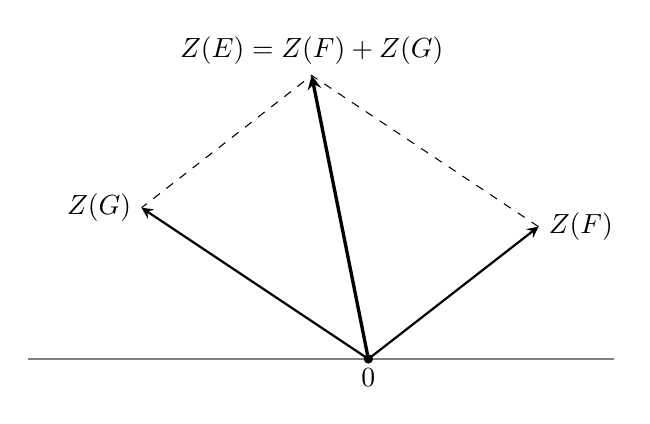
\begin{tikzpicture}[scale=1.2, >=stealth]
			% real axis
			\draw[gray] (-3.6,0) -- (2.6,0);
			\fill (0,0) circle (1.4pt) node[below] {$0$};
			% vectors
			\coordinate (F) at (1.8,1.4);
			\coordinate (G) at (-2.4,1.6);
			\coordinate (E) at (-0.6,3.0);
			\draw[thick, ->] (0,0) -- (F) node[right] {$Z(F)$};
			\draw[thick, ->] (0,0) -- (G) node[left] {$Z(G)$};
			\draw[very thick, ->] (0,0) -- (E) node[above] {$Z(E) = Z(F) + Z(G)$};
			% parallelogram
			\draw[dashed] (F) -- (E) -- (G);
		\end{tikzpicture}
	\end{center}
	The picture shows the case of a short exact sequence $0 \to F \to E \to G \to 0$:
	since $Z(F)$ and $Z(G)$ both lie in $\HH$, their sum $Z(E)$ lies in the sector between them,
	so the phase of $E$ is caught between the phases of $F$ and $G$.

	\begin{proof}
		By additivity, $Z(E) = \sum_j Z(B_j) = \sum_j r_j e^{i \pi \psi_j}$, where $r_j = m(B_j) > 0$ and $\psi_j = \varphi(B_j) \in (0, 1]$. Put $\psi := \max_j \psi_j$. Then
		\[
		e^{-i \pi \psi} Z(E) = \sum_j r_j e^{i \pi (\psi_j - \psi)}, \qquad \psi_j - \psi \in (-1, 0],
		\]
		so every summand has non-positive imaginary part, with equality if and only if $\psi_j = \psi$, in which case the summand is the positive real number $r_j$. 
		Hence $\im \big( e^{-i \pi \psi} Z(E) \big) \leqslant 0$, with equality if and only if all $\psi_j$ equal $\psi$. On the other hand $e^{-i \pi \psi} Z(E) = m(E) e^{i \pi \theta}$ with $\theta := \varphi(E) - \psi \in (-1, 1)$, and $\sin(\pi \theta) \leqslant 0$ on this interval exactly when $\theta \in (-1, 0]$, with $\sin(\pi \theta) = 0$ exactly when $\theta = 0$. This proves the upper bound and its equality case; the lower bound is obtained in the same way with $\min_j \psi_j$ in place of $\psi$.
		
		For a short exact sequence apply the above to the chain $0 \subset F \subset E$ with factors $F, G$: if, say, $\varphi(F) \leqslant \varphi(G)$, then $\varphi(F) \leqslant \varphi(E) \leqslant \varphi(G)$ and $\varphi(E)$ equals one of the endpoints only if $\varphi(F) = \varphi(G)$; the case $\varphi(F) \geqslant \varphi(G)$ is symmetric.
	\end{proof}
	
	\begin{lemma}[quotient characterization, {\cite[Exercise~4.4]{MS17}}]
		\label{lem:quotients}
		A nonzero object $E$ is $(\calA, Z)$-semistable 
		if and only if $\varphi(E) \leqslant \varphi(G)$ for every nonzero quotient $E \twoheadrightarrow G$, 
		and $(\calA, Z)$-stable if and only if $\varphi(E) < \varphi(G)$ for every nonzero proper quotient.
	\end{lemma}
	
	\begin{proof}
		Nontrivial proper subobjects $F \subset E$ correspond to nonzero proper quotients $G = E / F$, 
		and by Lemma~\ref{lem:seesaw} 
		the inequality $\varphi(F) \leqslant \varphi(E)$ is equivalent to $\varphi(E) \leqslant \varphi(G)$, 
		and similarly for strict inequalities. 
		The subobject $F = E$ and the quotient $G = E$ impose no condition.
	\end{proof}
	
	\begin{lemma}[Schur, {\cite[Thm~1]{Rud97}}, {\cite[Lemma~4.5]{MS17}}]
		\label{lem:schur}
		Let $E, F$ be $(\calA, Z)$-semistable objects.
		\begin{enumerate}
			\item If $\varphi(E) > \varphi(F)$, then $\Hom(E, F) = 0$.
			\item If $\varphi(E) = \varphi(F)$ and $f \colon E \to F$ is nonzero, then $f$ is a monomorphism provided $E$ is stable, an epimorphism provided $F$ is stable, and an isomorphism provided both are stable.
		\end{enumerate}
	\end{lemma}
	
	\begin{proof}
		Let $f \colon E \to F$ be nonzero, with image $I \neq 0$ and kernel $K$. 
		Since $I$ is a quotient of $E$, Lemma~\ref{lem:quotients} gives $\varphi(E) \leqslant \varphi(I)$; 
		since $I \subset F$, semistability of $F$ gives $\varphi(I) \leqslant \varphi(F)$. 
		Thus $\varphi(E) \leqslant \varphi(F)$, which proves (1). 
		In the situation of (2) all these inequalities are equalities. 
		If $E$ is stable and $K \neq 0$, 
		then $K$ is a nontrivial proper subobject of $E$ (proper because $I \neq 0$) and, 
		by Lemma~\ref{lem:seesaw} applied to 
		\[0 \to K \to E \to I \to 0, \] 
		$\varphi(E) = \varphi(I)$ forces $\varphi(K) = \varphi(E)$, contradicting stability; so $K = 0$. If $F$ is stable, then $I \subset F$ with $\varphi(I) = \varphi(F)$ forces $I = F$. The last claim combines the two.
	\end{proof}
	
	\begin{lemma}
		\label{lem:direct_sums}
		If $E$ and $F$ are $(\calA, Z)$-semistable of the same phase $\varphi$, then so is $E \oplus F$.
	\end{lemma}
	
	\begin{proof}
		First, 
		\[ Z(E \oplus F) = Z(E) + Z(F) \] 
		is a sum of two vectors on the ray $\RR_{>0} e^{i \pi \varphi}$, so $\varphi(E \oplus F) = \varphi$. Let $G \subset E \oplus F$ be nontrivial, and put $G' := \ker(G \to F) = G \cap E \subset E$ and $G'' := \image(G \to F) \subset F$, so that $0 \to G' \to G \to G'' \to 0$ is exact. If both $G'$ and $G''$ are nonzero, they have phases $\leqslant \varphi$ by semistability of $E$ and $F$, and Lemma~\ref{lem:seesaw} gives $\varphi(G) \leqslant \varphi$; if one of them vanishes, $G$ is isomorphic to the other and the same conclusion holds.
	\end{proof}
	
	\begin{lemma}
		\label{lem:hom_HN}
		Let $E, F$ be nonzero objects admitting HN filtrations, with HN factors $A_1, \ldots, A_n$ and $B_1, \ldots, B_m$ respectively. If $\Hom(E, F) \neq 0$, then $\varphi^-(E) \leqslant \varphi^+(F)$; more precisely, $\varphi(A_i) \leqslant \varphi(B_j)$ for some $i, j$.
	\end{lemma}
	
	\begin{proof}
		Let $f \colon E \to F$ be nonzero, and let $0 = E_0 \subset \ldots \subset E_n = E$, $0 = F_0 \subset \ldots \subset F_m = F$ be the filtrations. Let $i$ be minimal with $f|_{E_i} \neq 0$. Then $f|_{E_{i-1}} = 0$, so $f|_{E_i}$ factors through a nonzero map $g \colon A_i = E_i / E_{i-1} \to F$. Let $j$ be minimal with $\image g \subset F_j$. Then the composite $A_i \to F_j \to B_j = F_j / F_{j-1}$ is nonzero, since otherwise $\image g \subset F_{j-1}$. By Lemma~\ref{lem:schur}(1) applied to the semistable objects $A_i$ and $B_j$, $\varphi(A_i) \leqslant \varphi(B_j)$. Finally $\varphi^-(E) \leqslant \varphi(A_i)$ and $\varphi(B_j) \leqslant \varphi^+(F)$.
	\end{proof}
	
	
	\subsection{Uniqueness of Harder--Narasimhan filtrations}
	
	\begin{proposition}[{\cite[Thm~2]{Rud97}}, {\cite[Exercise~4.7]{MS17}}]
		\label{prop:HN_unique}
		Let $Z$ be a stability function on $\calA$ and let $E$ be a nonzero object. If
		\[
		0 = E_0 \subset E_1 \subset \ldots \subset E_n = E
		\qquad\text{and}\qquad
		0 = E'_0 \subset E'_1 \subset \ldots \subset E'_m = E
		\]
		are two HN filtrations of $E$ with respect to $(\calA, Z)$, then $n = m$ and $E_i = E'_i$ as subobjects of $E$ for all $i$. In particular the HN factors and the phases $\varphi^{\pm}(E)$ depend only on $E$.
	\end{proposition}
	
	\begin{proof}
		Write $A_i := E_i / E_{i-1}$, $\varphi_i := \varphi(A_i)$ and $A'_j := E'_j / E'_{j-1}$, $\varphi'_j := \varphi(A'_j)$. We argue by induction on $n$.
		
		\step{$E_1 = E'_1$} Let $j$ be minimal with $E_1 \subset E'_j$; it exists since $E'_m = E$. The composite $E_1 \to E'_j \to A'_j$ is nonzero, because otherwise $E_1 \subset E'_{j-1}$. Both $E_1 = A_1$ and $A'_j$ are semistable, so Lemma~\ref{lem:schur}(1) gives $\varphi_1 \leqslant \varphi'_j \leqslant \varphi'_1$. By symmetry $\varphi'_1 \leqslant \varphi_1$. Hence $\varphi_1 = \varphi'_1$, and then $\varphi'_j \geqslant \varphi'_1$ forces $j = 1$ because the phases $\varphi'_j$ strictly decrease; thus $E_1 \subset E'_1$. By symmetry $E'_1 \subset E_1$, so $E_1 = E'_1$.
		
		\step{induction} If $n = 1$, then $E = E_1 = E'_1$, so $m = 1$ as well. If $n > 1$, consider $\bar E := E / E_1 = E / E'_1 \neq 0$. The images $\bar E_i := E_i / E_1$, $i \geqslant 1$, form a chain $0 = \bar E_1 \subset \ldots \subset \bar E_n = \bar E$ with factors $\bar E_i / \bar E_{i-1} \cong E_i / E_{i-1} = A_i$ for $i \geqslant 2$, hence an HN filtration of $\bar E$ of length $n - 1$; similarly for $\bar E'_j := E'_j / E'_1$. By induction $n - 1 = m - 1$ and $\bar E_i = \bar E'_i$ for all $i \geqslant 1$. Since subobjects of $\bar E$ correspond bijectively to subobjects of $E$ containing $E_1 = E'_1$, we get $E_i = E'_i$ for all $i$.
	\end{proof}
	
	\begin{corollary}[{\cite[Prop.~1.9]{Rud97}}]
		\label{cor:HN_sub}
		Let $(\calA, Z)$ be a stability condition and $E$ a nonzero object. Then $\varphi^+(E) = \max \{ \varphi(F) : 0 \neq F \subset E \}$, and the first step $E_1$ of the HN filtration is the unique largest subobject of $E$ of phase $\varphi^+(E)$. Dually $\varphi^-(E) = \min \{ \varphi(G) : E \twoheadrightarrow G \neq 0 \}$.
	\end{corollary}
	
	\begin{proof}
		Let $0 \neq F \subset E$, with HN filtration $0 \subset F_1 \subset \ldots \subset F$. The composite $F_1 \hookrightarrow F \hookrightarrow E$ is a nonzero map from the semistable object $F_1$ to $E$, so Lemma~\ref{lem:hom_HN} gives $\varphi^+(F) = \varphi(F_1) \leqslant \varphi^+(E)$, and $\varphi(F) \leqslant \varphi^+(F)$ by Lemma~\ref{lem:seesaw}. The value $\varphi^+(E)$ is attained by $F = E_1$. Now suppose $\varphi(F) = \varphi^+(E)$. Then $\varphi(F) = \varphi^+(F)$, so by the equality case of Lemma~\ref{lem:seesaw} all HN factors of $F$ have phase $\varphi^+(E)$, i.e.\ $F$ is semistable of phase $\varphi^+(E)$. All HN factors of $E / E_1$ have phase $< \varphi^+(E)$, so the composite $F \to E \to E / E_1$ vanishes by Lemma~\ref{lem:hom_HN}, i.e.\ $F \subset E_1$. The dual statement follows by the same argument applied to quotients, using Lemma~\ref{lem:quotients}.
	\end{proof}
	
	
	\subsection{Existence of Harder--Narasimhan filtrations}
	
	Recall that an abelian category $\calA$ is \emph{noetherian} if every ascending chain $F_1 \subset F_2 \subset \ldots$ of subobjects of any object stabilizes.
	Equivalently, every nonempty family of subobjects of an object has a maximal element with respect to inclusion.
	Throughout this subsection $Z$ is a stability function on $\calA$, and we write $R := \im Z$ and $D := -\re Z$, so that $R(F) \geqslant 0$ for all $F$, and $R(F) = 0$ implies $D(F) > 0$ for $F \neq 0$.
	We say that \emph{$R$ has discrete image} if $R(\Kgroup(\calA))$ is a discrete subgroup of $\RR$;
	in that case either $R \equiv 0$, or $R(\Kgroup(\calA)) = c \ZZ$ for a unique $c > 0$, and then $R(E) \in c \ZZ_{\geqslant 0}$ for every object $E$.
	
	Two elementary identities will be used repeatedly.
	If $F, F' \subset E$ are subobjects, the sequence
	\[
	0 \to F \cap F' \to F \oplus F' \to F + F' \to 0
	\]
	is exact, hence
	\begin{equation}
		\label{eq:modular}
		Z(F + F') + Z(F \cap F') = Z(F) + Z(F') ,
	\end{equation}
	and the same holds for $R$ and $D$ separately.
	If $F \subset E$ and $R(F) = R(E)$, then $R(E / F) = 0$, so $D(E / F) \geqslant 0$ and
	\begin{equation}
		\label{eq:same_rank}
		D(F) \leqslant D(E) \qquad \text{whenever } F \subset E \text{ and } R(F) = R(E).
	\end{equation}
	
	\begin{lemma}[{\cite[Lemma~4.9]{MS17}}]
		\label{lem:D_bounded}
		Assume that
		\begin{itemize}
			\item $\calA$ is noetherian and
			\item that $R$ has discrete image in $ \mathbb{R} $.
		\end{itemize}
		Then for every object $E$ there is a constant $D_E \in \RR$ such that $D(F) \leqslant D_E$ for every subobject $F \subset E$.
	\end{lemma}
	
	\begin{proof}
		If $R \equiv 0$, then every $F \subset E$ satisfies $R(F) = R(E)$ and \eqref{eq:same_rank} gives $D(F) \leqslant D(E)$.
		Otherwise write $R(\Kgroup(\calA)) = c \ZZ$ with $c > 0$ and argue by induction on $k(E) := R(E) / c \in \ZZ_{\geqslant 0}$.
		
		If $k(E) = 0$, then $R(F) = 0 = R(E)$ for every $F \subset E$, and \eqref{eq:same_rank} gives $D(F) \leqslant D(E)$.
		
		Let $k(E) > 0$ and assume the lemma for all objects $E'$ with $k(E') < k(E)$.
		Suppose, for a contradiction, that there are subobjects $F_n \subset E$, $n \in \ZZ_{>0}$, with $D(F_n) \to \infty$.
		By \eqref{eq:same_rank} only finitely many of them can satisfy $R(F_n) = R(E)$, so after discarding these we may assume $R(F_n) < R(E)$ for all $n$.
		We construct indices $n_1 < n_2 < \ldots$ such that the subobjects $G_k := F_{n_1} + \ldots + F_{n_k}$ satisfy
		\[
		R(G_k) < R(E)
		\qquad\text{and}\qquad
		D(G_k) > D(G_{k-1}) \quad (k \geqslant 2).
		\]
		Put $n_1 := 1$.
		Given $n_1 < \ldots < n_{k-1}$, the object $G_{k-1}$ satisfies $k(G_{k-1}) < k(E)$, so by the induction hypothesis there is a constant $D'$ with $D(F') \leqslant D'$ for all $F' \subset G_{k-1}$.
		For $n > n_{k-1}$, identity \eqref{eq:modular} and $G_{k-1} \cap F_n \subset G_{k-1}$ give
		\[
		D(G_{k-1} + F_n) = D(G_{k-1}) + D(F_n) - D(G_{k-1} \cap F_n) \geqslant D(G_{k-1}) + D(F_n) - D' ,
		\]
		which tends to $\infty$ as $n \to \infty$.
		Choose $n_k > n_{k-1}$ with 
		\[
		D(G_{k-1} + F_{n_k}) > \max \{ D(E), D(G_{k-1}) \}.
		\]
		Then $R(G_{k-1} + F_{n_k}) < R(E)$ by \eqref{eq:same_rank}, and $D(G_k) > D(G_{k-1})$ as required.
		Since $D(G_k) > D(G_{k-1})$, the inclusion $G_{k-1} \subset G_k$ is strict, so $G_1 \subsetneq G_2 \subsetneq \ldots$ is an infinite strictly ascending chain of subobjects of $E$, contradicting noetherianity.
	\end{proof}
	
	\begin{proposition}[{\cite[Prop.~4.10]{MS17}}; cf.\ {\cite[Thm~2]{Rud97}}, {\cite[Prop.~2.4]{Bri07}}]
		\label{prop:HN_existence}
		Let $Z$ be a stability function on $\calA$.
		Assume that $\calA$ is noetherian and that $R = \im Z$ has discrete image.
		Then every nonzero object of $\calA$ admits a Harder--Narasimhan filtration, i.e.\ $(\calA, Z)$ is a stability condition.
	\end{proposition}
	
	\begin{proof}
		If $R \equiv 0$, then every nonzero object has phase $1$, every nonzero object is semistable, and $0 \subset E$ is an HN filtration.
		So assume $R(\Kgroup(\calA)) = c \ZZ$ with $c > 0$, and let $E \neq 0$.
		
		\step{the part of rank zero}
		The family of subobjects $F \subset E$ with $R(F) = 0$ is nonempty (it contains $0$), so it has a maximal element $T$.
		If $F \subset E$ is any subobject with $R(F) = 0$, then $R(T + F) = R(T) + R(F) - R(T \cap F) = -R(T \cap F) \leqslant 0$ by \eqref{eq:modular}, hence $R(T + F) = 0$ and $T + F = T$ by maximality, i.e.\ $F \subset T$.
		Thus $T$ is the largest subobject of $E$ of rank zero.
		If $T \neq 0$, it is semistable of phase $1$, because all its nonzero subobjects have $R = 0$, hence phase $1$.
		Moreover the quotient $\bar E := E / T$ has no nonzero subobject of rank zero:
		the preimage $F \subset E$ of such a subobject $\bar F$ satisfies $R(F) = R(T) + R(\bar F) = 0$, hence $F \subset T$ and $\bar F = 0$.
		Consequently every nonzero subobject of $\bar E$ has $R \geqslant c$, hence phase $< 1$.
		If $\bar E = 0$, then $E = T$ is semistable and we are done.
		Otherwise, if $0 = \bar E_0 \subset \bar E_1 \subset \ldots \subset \bar E_m = \bar E$ is an HN filtration of $\bar E$, then its factors have phases $< 1$, and the preimages
		\[
		0 \subset T \subset \pi^{-1}(\bar E_1) \subset \ldots \subset \pi^{-1}(\bar E_m) = E
		\]
		form an HN filtration of $E$ (with the first step omitted if $T = 0$), since the factors are $T$ (of phase $1$) followed by the factors of the filtration of $\bar E$.
		Hence we may and do assume from now on that
		\begin{equation}
			\label{eq:no_torsion}
			\text{every nonzero subobject } F \subset E \text{ satisfies } R(F) \geqslant c .
		\end{equation}
		\begin{illustration}
		In the pictures accompanying this proof we draw the plane of $Z$ in the usual way, with $\re Z$ to the right and $\im Z$ upwards;
		a subobject $F \subset E$ is represented by the point $Z(F)$, whose height is the rank $R(F)$ and whose degree $D(F) = -\re Z(F)$ grows to the left, so that the point with coordinates $(R, D) = (r, d)$ in the proof is the point $-d + i r$ of the plane.
		In Step~1, the subobjects of rank zero are the points on the negative real axis, $T$ is the leftmost of them, and passing from $E$ to $\bar E = E / T$ shifts every point to the right by $D(T)$.
		\begin{center}
			\begin{tikzpicture}[scale=1.0, >=stealth, rotate=90]
				\draw[->, gray] (0,3.4) -- (0,-0.6) node[right] {$\re$};
				\draw[->, gray] (-0.3,0) -- (4.6,0) node[above] {$\im$};
				\foreach \y in {0.4, 0.9, 1.3}
					\fill[gray] (0,\y) circle (1.1pt);
				\fill (0,1.7) circle (1.6pt) node[below] {$Z(T)$};
				\fill (0,0) circle (1.4pt) node[below right] {$0$};
				\fill (3.6,2.9) circle (1.6pt) node[left] {$Z(E)$};
				\fill (3.6,1.2) circle (1.6pt) node[right] {$Z(\bar E)$};
				\draw[->, dashed] (3.6,2.75) -- (3.6,1.35) node[midway, above, font=\footnotesize] {$D(T)$};
				\draw[dotted] (0,1.7) -- (3.6,1.7);
			\end{tikzpicture}
		\end{center}
		\end{illustration}
		
		\step{the Harder--Narasimhan polygon}
		For $r \in c \ZZ$ with $0 \leqslant r \leqslant R(E)$ let $\mathcal{S}_r$ be the set of subobjects $F \subset E$ with $R(F) = r$, and call $r$ \emph{occupied} if $\mathcal{S}_r \neq \emptyset$.
		The set $\Lambda_E$ of occupied values is finite and contains $0$ and $R(E)$.
		For $r \in \Lambda_E$ put
		\[
		d(r) := \sup \{ D(F) : F \in \mathcal{S}_r \} ,
		\]
		which is finite by Lemma~\ref{lem:D_bounded}.
		By \eqref{eq:no_torsion} we have $\mathcal{S}_0 = \{ 0 \}$ and $d(0) = 0$, and by \eqref{eq:same_rank} we have $d(R(E)) = D(E)$, attained by $E$ itself.
		Let $p \colon [0, R(E)] \to \RR$ be the upper concave envelope of the finite set of points $(r, d(r))$, $r \in \Lambda_E$, i.e.\ the smallest concave function with $p(r) \geqslant d(r)$ for all $r \in \Lambda_E$.
		It is piecewise linear, and its graph is the upper boundary of the convex hull of these points.
		Let $0 = r_0 < r_1 < \ldots < r_n = R(E)$ be the endpoints together with the points where the slope of $p$ changes; we call them the \emph{vertices}.
		They belong to $\Lambda_E$, satisfy $p(r_i) = d(r_i) =: d_i$, and the slopes
		\[
		s_i := \frac{d_i - d_{i-1}}{r_i - r_{i-1}} , \qquad i = 1, \ldots, n ,
		\]
		are strictly decreasing, $s_1 > s_2 > \ldots > s_n$, because $p$ is concave and changes slope at every $r_i$ with $0 < i < n$.
		On $[r_{i-1}, r_i]$ the function $p$ is affine with slope $s_i$.
		Finally, for every subobject $F \subset E$ we have $R(F) \in \Lambda_E$ and
		\begin{equation}
			\label{eq:below_p}
			D(F) \leqslant d(R(F)) \leqslant p(R(F)) .
		\end{equation}
		\begin{illustration}
		The picture below shows the sets $\mathcal{S}_r$ as horizontal rows of points at the occupied heights $r \in \Lambda_E$, the suprema $d(r)$ as the leftmost points of the rows (a hollow circle marks a supremum which is not attained), the graph of the envelope $p$ as the thick line, and the vertices $r_0, \ldots, r_n$ as the heights at which this line bends;
		concavity of $p$ means that the line bends to the right as one goes up.
		\begin{center}
			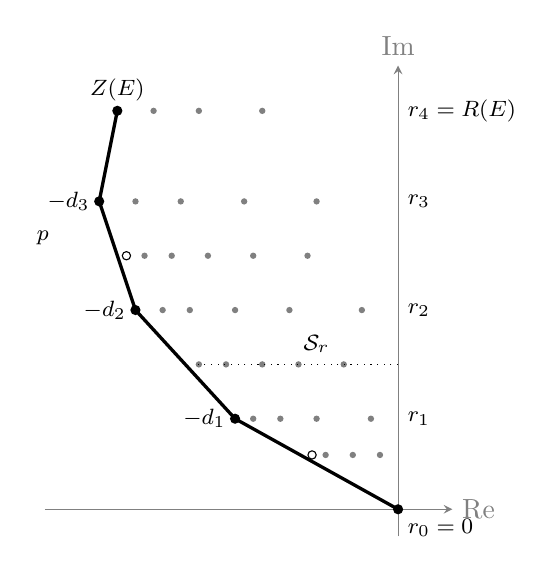
\begin{tikzpicture}[scale=1.15, >=stealth, rotate=90]
				% axes of the plane of Z: real axis to the right, imaginary axis upwards
				\draw[->, gray] (0,3.9) -- (0,-0.6) node[right] {$\re$};
				\draw[->, gray] (-0.3,0) -- (4.9,0) node[above] {$\im$};
				\foreach \x/\ys in {0.6/{0.2,0.5,0.8}, 1/{0.3,0.9,1.3,1.6}, 1.6/{0.6,1.1,1.5,1.9,2.2}, 2.2/{0.4,1.2,1.8,2.3,2.6}, 2.8/{1.0,1.6,2.1,2.5,2.8}, 3.4/{0.9,1.7,2.4,2.9}, 4.4/{1.5,2.2,2.7}}
					\foreach \y in \ys
						\fill[gray] (\x,\y) circle (1.0pt);
				\draw (0.6,0.95) circle (1.3pt);
				\draw (2.8,3.0) circle (1.3pt);
				\coordinate (v0) at (0,0);
				\coordinate (v1) at (1,1.8);
				\coordinate (v2) at (2.2,2.9);
				\coordinate (v3) at (3.4,3.3);
				\coordinate (v4) at (4.4,3.1);
				\draw[very thick] (v0) -- (v1) -- (v2) -- (v3) -- (v4);
				\foreach \v in {v0,v1,v2,v3,v4} \fill (\v) circle (1.6pt);
				\node[below right, font=\footnotesize] at (0,0) {$r_0 = 0$};
				\node[right, font=\footnotesize] at (1,0) {$r_1$};
				\node[right, font=\footnotesize] at (2.2,0) {$r_2$};
				\node[right, font=\footnotesize] at (3.4,0) {$r_3$};
				\node[right, font=\footnotesize] at (4.4,0) {$r_4 = R(E)$};
				\node[left, font=\footnotesize] at (v1) {$-d_1$};
				\node[left, font=\footnotesize] at (v2) {$-d_2$};
				\node[left, font=\footnotesize] at (v3) {$-d_3$};
				\node[above, font=\footnotesize] at (v4) {$Z(E)$};
				\node[above, font=\footnotesize] at (1.62,0.9) {$\mathcal{S}_{r}$};
				\draw[dotted] (1.6,0) -- (1.6,2.25);
				\node[left, font=\footnotesize] at (3.0,3.75) {$p$};
			\end{tikzpicture}
		\end{center}
		Note that a non-vertex height may well be occupied (the row along the dotted line in the picture); what makes $r_i$ a vertex is that the line bends there.
		\end{illustration}
		
		\step{the suprema at the vertices are attained}
		We claim that for every vertex $r_i$ there is $F_i \in \mathcal{S}_{r_i}$ with $D(F_i) = d_i$ (this is \cite[Exercise~4.11]{MS17}).
		For $i = 0$ take $F_0 = 0$ and for $i = n$ take $F_n = E$.
		Let $0 < i < n$ and choose a number $s$ with $s_i > s > s_{i+1}$.
		Consider the linear functional $\ell(x, y) := y - s x$ on $\RR^2$ and put $M := \ell(r_i, d_i) = d_i - s r_i$.
		Since $s$ lies between the slopes of $p$ to the left and to the right of $r_i$, concavity gives $p(x) \leqslant d_i + s (x - r_i)$ for all $x \in [0, R(E)]$, with equality only for $x = r_i$.
		Together with \eqref{eq:below_p} this shows
		\begin{equation}
			\label{eq:ell_bound}
			\ell\big( R(F), D(F) \big) \leqslant M \qquad \text{for every subobject } F \subset E ,
		\end{equation}
		and moreover, since $\Lambda_E$ is finite,
		\[
		\gamma := M - \max \big\{ p(r) - s r : r \in \Lambda_E,\ r \neq r_i \big\} > 0 ,
		\]
		so that $\ell(R(F), D(F)) > M - \gamma$ forces $R(F) = r_i$.
		\begin{illustration}
		The picture shows the line through the vertex $Z(F_i) = -d_i + i r_i$ corresponding to the slope $s$: it is a supporting line of the polygon, touching it only at that vertex, so all points $Z(F)$ lie on it or to the right of it, and the points of the other rows stay to the right of the dashed parallel line, at horizontal distance $\gamma$ from the first one; only the points of the row $\mathcal{S}_{r_i}$ can come arbitrarily close to the solid line.
		\begin{center}
			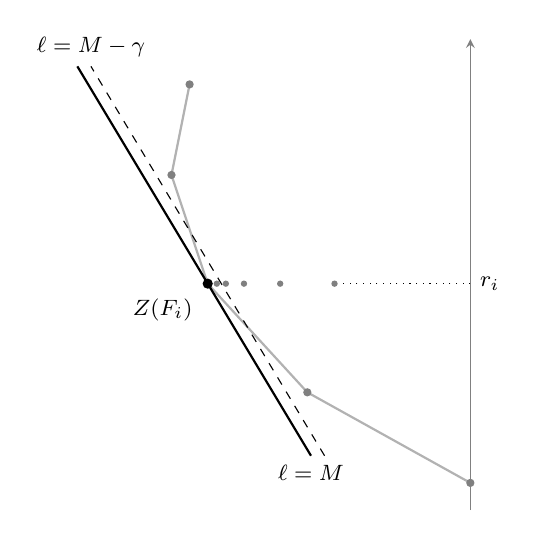
\begin{tikzpicture}[scale=1.15, >=stealth, rotate=90]
				\coordinate (v0) at (0,0);
				\coordinate (v1) at (1,1.8);
				\coordinate (v2) at (2.2,2.9);
				\coordinate (v3) at (3.4,3.3);
				\coordinate (v4) at (4.4,3.1);
				\draw[thick, gray!60] (v0) -- (v1) -- (v2) -- (v3) -- (v4);
				\draw[thick] (0.3,1.76) -- (4.6,4.34);
				\node[below, font=\footnotesize] at (0.3,1.76) {$\ell = M$};
				\draw[dashed] (0.3,1.61) -- (4.6,4.19);
				\node[above, font=\footnotesize] at (4.6,4.19) {$\ell = M - \gamma$};
				\foreach \y in {1.5, 2.1, 2.5, 2.7, 2.8}
					\fill[gray] (2.2,\y) circle (1.0pt);
				\fill (v2) circle (1.6pt);
				\node[below left=2pt, font=\footnotesize] at (v2) {$Z(F_i)$};
				\foreach \v in {v0,v1,v3,v4} \fill[gray] (\v) circle (1.3pt);
				\draw[->, gray] (-0.3,0) -- (4.9,0);
				\node[right, font=\footnotesize] at (2.2,0) {$r_i$};
				\draw[dotted] (2.2,0) -- (2.2,1.45);
			\end{tikzpicture}
		\end{center}
		\end{illustration}
		For brevity write $\ell(F) := \ell(R(F), D(F))$.
		Applying $\ell$ to \eqref{eq:modular} and using \eqref{eq:ell_bound} for $F \cap F'$ we get, for all $F, F' \subset E$,
		\begin{equation}
			\label{eq:ell_sum}
			\ell(F + F') = \ell(F) + \ell(F') - \ell(F \cap F') \geqslant \ell(F) + \ell(F') - M .
		\end{equation}
		Now choose $F^{(1)}, F^{(2)}, \ldots \in \mathcal{S}_{r_i}$ with $D(F^{(j)}) \to d_i$, and put $\varepsilon_j := M - \ell(F^{(j)}) = d_i - D(F^{(j)}) \geqslant 0$.
		Passing to a subsequence we may assume $\sum_j \varepsilon_j < \gamma$.
		Let $G_k := F^{(1)} + \ldots + F^{(k)}$.
		By induction on $k$, \eqref{eq:ell_sum} gives
		\[
		\ell(G_k) \geqslant \sum_{j=1}^{k} \ell(F^{(j)}) - (k-1) M = M - \sum_{j=1}^{k} \varepsilon_j > M - \gamma .
		\]
		The chain $G_1 \subset G_2 \subset \ldots$ stabilizes by noetherianity, say $G_k = G$ for $k \geqslant N$.
		Then $\ell(G) > M - \gamma$, hence $R(G) = r_i$, and $G \supset F^{(j)}$ for every $j$.
		For $j \geqslant N$ the quotient $G / F^{(j)}$ has $R(G / F^{(j)}) = r_i - r_i = 0$, so $D(G / F^{(j)}) \geqslant 0$ and $D(G) \geqslant D(F^{(j)})$.
		Letting $j \to \infty$ we obtain $D(G) \geqslant d_i$, hence $D(G) = d_i$ by definition of $d_i$.
		Thus $F_i := G$ has the required property.
		
		\step{the vertices form a chain}
		Fix $1 \leqslant i \leqslant n$ and consider the functional $\ell_i(x, y) := y - s_i x$ and the number $M_i := \ell_i(r_{i-1}, d_{i-1}) = \ell_i(r_i, d_i)$.
		By concavity, $p(x) \leqslant d_{i-1} + s_i (x - r_{i-1})$ for all $x$, with equality exactly for $x \in [r_{i-1}, r_i]$, because the slope of $p$ is $> s_i$ to the left of $r_{i-1}$ and $< s_i$ to the right of $r_i$.
		Hence, by \eqref{eq:below_p}, $\ell_i(F) \leqslant M_i$ for every $F \subset E$, and $\ell_i(F) = M_i$ implies $r_{i-1} \leqslant R(F) \leqslant r_i$ and $D(F) = p(R(F))$.
		Apply \eqref{eq:modular} to $F_{i-1}$ and $F_i$:
		\[
		\ell_i(F_{i-1} \cap F_i) + \ell_i(F_{i-1} + F_i) = \ell_i(F_{i-1}) + \ell_i(F_i) = 2 M_i .
		\]
		Both summands on the left are $\leqslant M_i$, so both equal $M_i$.
		\begin{illustration}
		In the picture, the points $Z(F_{i-1} \cap F_i)$ and $Z(F_{i-1} + F_i)$ are symmetric with respect to the midpoint of the edge from $Z(F_{i-1})$ to $Z(F_i)$ by \eqref{eq:modular}, and both must lie on the line $\ell_i = M_i$ carrying that edge or to the right of it; the dashed configuration is therefore impossible, and both points are forced onto the line, hence onto the edge.
		\begin{center}
			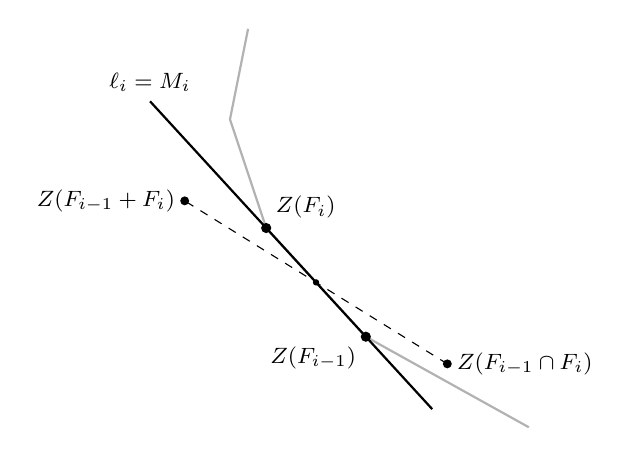
\begin{tikzpicture}[scale=1.15, >=stealth, rotate=90]
				\coordinate (v0) at (0,0);
				\coordinate (v1) at (1,1.8);
				\coordinate (v2) at (2.2,2.9);
				\coordinate (v3) at (3.4,3.3);
				\coordinate (v4) at (4.4,3.1);
				\draw[thick, gray!60] (v0) -- (v1) -- (v2) -- (v3) -- (v4);
				\draw[thick] (0.2,1.0667) -- (3.6,4.1833);
				\node[above, font=\footnotesize] at (3.6,4.1833) {$\ell_i = M_i$};
				\fill (v1) circle (1.6pt) node[below left, font=\footnotesize] {$Z(F_{i-1})$};
				\fill (v2) circle (1.6pt) node[above right, font=\footnotesize] {$Z(F_i)$};
				\coordinate (cap) at (0.7,0.9);
				\coordinate (sum) at (2.5,3.8);
				\fill (cap) circle (1.4pt) node[right, font=\footnotesize] {$Z(F_{i-1} \cap F_i)$};
				\fill (sum) circle (1.4pt) node[left, font=\footnotesize] {$Z(F_{i-1} + F_i)$};
				\draw[dashed] (cap) -- (sum);
				\fill (1.6,2.35) circle (1.0pt);
			\end{tikzpicture}
		\end{center}
		\end{illustration}
		Since $R(F_{i-1} \cap F_i) \leqslant R(F_{i-1}) = r_{i-1}$, the first equality forces $R(F_{i-1} \cap F_i) = r_{i-1}$ and $D(F_{i-1} \cap F_i) = p(r_{i-1}) = d_{i-1} = D(F_{i-1})$.
		Therefore the quotient $F_{i-1} / (F_{i-1} \cap F_i)$ has $R = 0$ and $D = 0$, i.e.\ $Z = 0$, so it is zero by \condref{cond:Z}.
		Hence $F_{i-1} \subset F_i$.
		We have obtained a chain
		\[
		0 = F_0 \subset F_1 \subset \ldots \subset F_n = E .
		\]
		
		\step{the factors are semistable with strictly decreasing phases}
		Put $A_i := F_i / F_{i-1}$.
		Then $Z(A_i) = Z(F_i) - Z(F_{i-1})$, i.e.\ $R(A_i) = r_i - r_{i-1} > 0$ and $D(A_i) = d_i - d_{i-1}$, so $A_i \neq 0$ and its generalized slope is $M(A_i) = s_i$.
		Since $s_1 > \ldots > s_n$, the phases of the $A_i$ strictly decrease.
		It remains to show that $A_i$ is semistable.
		Let $S \subset A_i$ be a nontrivial subobject and $F' \subset F_i$ its preimage, so that $F_{i-1} \subsetneq F' \subset F_i$ and $Z(S) = Z(F') - Z(F_{i-1})$.
		Then $r_{i-1} \leqslant R(F') \leqslant r_i$, because $R(F' / F_{i-1}) \geqslant 0$ and $R(F_i / F') \geqslant 0$, and \eqref{eq:below_p} together with the affine form of $p$ on $[r_{i-1}, r_i]$ gives
		\[
		D(F') \leqslant p(R(F')) = d_{i-1} + s_i \big( R(F') - r_{i-1} \big) .
		\]
		In other words $D(S) \leqslant s_i R(S)$.
		\begin{illustration}
		In the picture, the point $Z(F')$ lies in the shaded horizontal strip $r_{i-1} \leqslant \im \leqslant r_i$ and on the edge of the polygon or to the right of it; hence the vector from $Z(F_{i-1})$ to $Z(F')$, which is $Z(S)$ for $S = F' / F_{i-1}$, has slope at most $s_i$, i.e.\ phase at most $\varphi(A_i)$.
		\begin{center}
			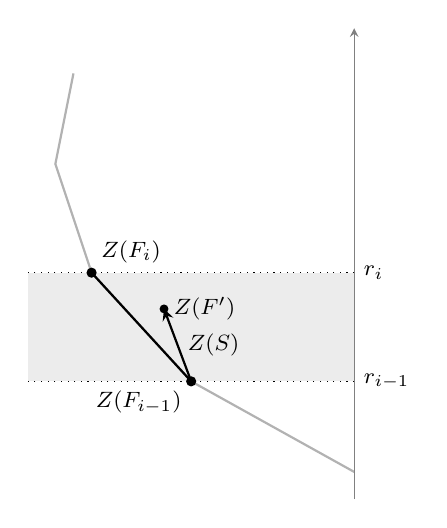
\begin{tikzpicture}[scale=1.15, >=stealth, rotate=90]
				\coordinate (v0) at (0,0);
				\coordinate (v1) at (1,1.8);
				\coordinate (v2) at (2.2,2.9);
				\coordinate (v3) at (3.4,3.3);
				\coordinate (v4) at (4.4,3.1);
				\fill[gray!15] (1,0) rectangle (2.2,3.6);
				\draw[thick, gray!60] (v0) -- (v1) -- (v2) -- (v3) -- (v4);
				\draw[thick] (v1) -- (v2);
				\fill (v1) circle (1.6pt) node[below left, font=\footnotesize] {$Z(F_{i-1})$};
				\fill (v2) circle (1.6pt) node[above right, font=\footnotesize] {$Z(F_i)$};
				\coordinate (fp) at (1.8,2.1);
				\fill (fp) circle (1.4pt) node[right, font=\footnotesize] {$Z(F')$};
				\draw[->, thick] (v1) -- (fp) node[midway, right, font=\footnotesize] {$Z(S)$};
				\draw[->, gray] (-0.3,0) -- (4.9,0);
				\node[right, font=\footnotesize] at (1,0) {$r_{i-1}$};
				\node[right, font=\footnotesize] at (2.2,0) {$r_i$};
				\draw[dotted] (1,0) -- (1,3.6);
				\draw[dotted] (2.2,0) -- (2.2,3.6);
			\end{tikzpicture}
		\end{center}
		\end{illustration}
		If $R(S) = 0$ this would give $D(S) \leqslant 0$, which is impossible for the nonzero object $S$; so $R(S) > 0$ and $M(S) = D(S) / R(S) \leqslant s_i = M(A_i)$, i.e.\ $\varphi(S) \leqslant \varphi(A_i)$.
		Thus $A_i$ is semistable, and $0 = F_0 \subset \ldots \subset F_n = E$ is an HN filtration of $E$.
	\end{proof}
	
	The proof shows that the HN filtration can be read off from the \emph{Harder--Narasimhan polygon} of $E$:
	the part of the boundary of the convex hull of $\{ Z(F) : F \subset E \}$ lying to the left of the segment from $0$ to $Z(E)$.
	Its vertices are the points $Z(F_i)$ and its edges are the vectors $Z(A_i)$.
	In the picture below the grey dots are the values $Z(F)$ of other subobjects $F \subset E$, the dashed segment joins $0$ to $Z(E)$, and the thick polygonal line is the HN polygon.
	
	\begin{center}
		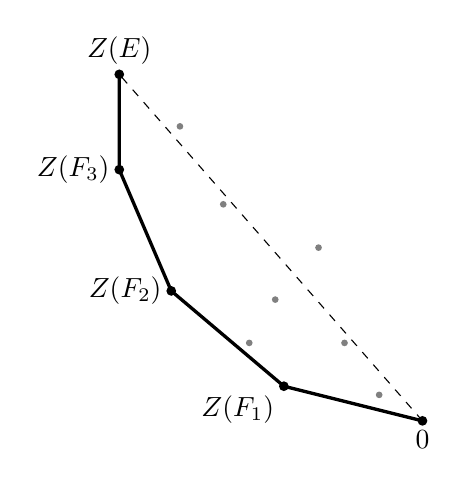
\begin{tikzpicture}[scale=1.1, >=stealth]
			\coordinate (v0) at (0,0);
			\coordinate (v1) at (-1.6,0.4);
			\coordinate (v2) at (-2.9,1.5);
			\coordinate (v3) at (-3.5,2.9);
			\coordinate (v4) at (-3.5,4.0);
			% some points Z(F) inside the hull
			\foreach \pt in {(-0.9,0.9), (-1.7,1.4), (-2.3,2.5), (-1.2,2.0), (-2.8,3.4), (-0.5,0.3), (-2.0,0.9)}
			\fill[gray] \pt circle (1.1pt);
			% chord
			\draw[dashed] (v0) -- (v4);
			% polygon
			\draw[very thick] (v0) -- (v1) -- (v2) -- (v3) -- (v4);
			\fill (v0) circle (1.6pt) node[below] {$0$};
			\fill (v1) circle (1.6pt) node[below left] {$Z(F_1)$};
			\fill (v2) circle (1.6pt) node[left] {$Z(F_2)$};
			\fill (v3) circle (1.6pt) node[left] {$Z(F_3)$};
			\fill (v4) circle (1.6pt) node[above] {$Z(E)$};
		\end{tikzpicture}
	\end{center}
	
	\begin{corollary}[Harder--Narasimhan \cite{HN75}]
		\label{cor:HN_curves}
		Let $C$ be a smooth projective curve over a field $\kk$ and $Z(E) = -\deg E + i \operatorname{rk} E$ on $\mathrm{Coh}(C)$.
		Then $(\mathrm{Coh}(C), Z)$ is a stability condition.
	\end{corollary}
	
	\begin{proof}
		$\mathrm{Coh}(C)$ is noetherian and $R = \operatorname{rk}$ takes values in $\ZZ$, so Proposition~\ref{prop:HN_existence} applies.
	\end{proof}
	
	\begin{remark}
		The proposition does not cover Example~\ref{ex:finite_dim_algebra} in general, since there $\im Z$ need not have discrete image; that example was treated by a direct finite-length argument.
		Bridgeland's original formulation \cite[Prop.~2.4]{Bri07} replaces the two hypotheses by two chain conditions on phases, which cover both situations at once;
		noetherianity excludes infinite descending chains of quotients with decreasing phases, and discreteness of $R$ excludes infinite descending chains of subobjects with increasing phases.
	\end{remark}
	
	
	\subsection{Examples}
	
	\begin{example}
		Let $C$ be a smooth projective curve over a field $\kk$, $\calA = \mathrm{Coh}(C)$, and
		\[
		Z(E) := -\deg E + i \operatorname{rk} E .
		\]
		This is a stability function: for a nonzero sheaf $E$ either $\operatorname{rk} E > 0$, or $E$ is a torsion sheaf, in which case $\deg E$ is the length of $E$, which is positive, so $Z(E) \in \RR_{<0}$. For $\operatorname{rk} E > 0$ the generalized slope $M(E) = \deg E / \operatorname{rk} E$ is the usual slope, and torsion sheaves have $M = +\infty$; thus $(\calA, Z)$-(semi)stability is slope (semi)stability, and semistable sheaves of positive rank are torsion-free. The Harder--Narasimhan property is Corollary~\ref{cor:HN_curves}, originally due to Harder and Narasimhan \cite{HN75}; the convex-polygon proof goes back to Shatz \cite{Sha77}. So $(\mathrm{Coh}(C), Z)$ is a stability condition.
	\end{example}
	
	\begin{example}
		Let $X$ be a smooth projective variety of dimension $n \geqslant 2$ and $\omega$ an ample divisor class. The homomorphism $Z(E) := -\omega^{n-1} \cdot c_1(E) + i \, \omega^n \cdot \operatorname{rk} E$ on $\Kgroup(\mathrm{Coh}(X))$ is not a stability function: for a nonzero sheaf $T$ supported in codimension $\geqslant 2$ both $\operatorname{rk} T$ and $c_1(T)$ vanish, so $Z(T) = 0 \notin \HH$. One can show that no homomorphism factoring through the Chern character is a stability function on $\mathrm{Coh}(X)$ (see \cite[Example~4.3]{MS17}, where this is deduced from \cite[Lemma~2.7]{Tod09}); this is the reason for passing to other hearts in the derived category.
	\end{example}
	
	\begin{example}[{\cite[Exercise~4.13]{MS17}}]
		\label{ex:finite_dim_algebra}
		Let $A$ be a finite-dimensional algebra over a field $\kk$, $\calA = \operatorname{mod}\text{-}A$ the category of finite-dimensional right $A$-modules, and $S_1, \ldots, S_m$ representatives of the isomorphism classes of simple modules. Every $M \in \calA$ has a composition series, and by the Jordan--H\"older theorem the multiplicity $[M : S_j]$ of $S_j$ among its factors is well defined and additive in short exact sequences. Hence
		\[
		\Kgroup(\calA) \longrightarrow \ZZ^m, \qquad [M] \longmapsto \big( [M : S_1], \ldots, [M : S_m] \big)
		\]
		is a well-defined homomorphism; it is surjective, and it is injective because every class $[M]$ equals $\sum_j [M : S_j] [S_j]$. So $[S_1], \ldots, [S_m]$ form a basis of $\Kgroup(\calA) \cong \ZZ^m$, and for any $z_1, \ldots, z_m \in \CC$ there is a unique homomorphism $Z$ with $Z(S_j) = z_j$, namely $Z(M) = \sum_j [M : S_j] z_j$.
		
		Now let $z_1, \ldots, z_m \in \HH$. Then $Z$ is a stability function, since $Z(M)$ is a sum of vectors in $\HH$ with non-negative coefficients, not all zero. We claim that $(\calA, Z)$ is a stability condition. Let $M \neq 0$; we construct an HN filtration by induction on the length $\ell(M)$.
		
		For a subobject $N \subset M$ one has $0 \leqslant [N : S_j] \leqslant [M : S_j]$, so the classes $[N]$, hence the phases $\varphi(N)$, range over a finite set. Let $\varphi_1$ be the maximal phase of a nontrivial subobject, and among the nontrivial subobjects of phase $\varphi_1$ choose $M_1$ of maximal length. Then $M_1$ is semistable: its subobjects are subobjects of $M$, hence have phase $\leqslant \varphi_1$. Moreover every nontrivial $N \subset M$ with $\varphi(N) = \varphi_1$ satisfies $N \subset M_1$. Indeed, from the exact sequence
		\[
		0 \to M_1 \cap N \to M_1 \oplus N \to M_1 + N \to 0
		\]
		and Lemma~\ref{lem:direct_sums}, $\varphi(M_1 \oplus N) = \varphi_1$, while $\varphi(M_1 \cap N) \leqslant \varphi_1$ if $M_1 \cap N \neq 0$; so Lemma~\ref{lem:seesaw} gives $\varphi(M_1 + N) \geqslant \varphi_1$, hence $= \varphi_1$ by maximality of $\varphi_1$. By maximality of $\ell(M_1)$, $\ell(M_1 + N) \leqslant \ell(M_1)$, so $M_1 + N = M_1$. (If $M_1 \cap N = 0$, then $M_1 + N \cong M_1 \oplus N$ has phase $\varphi_1$ and larger length, which is impossible, so this case does not occur.)
		
		Finally, every nontrivial subobject $N' \subset M / M_1$ has $\varphi(N') < \varphi_1$: if $N \subset M$ is its preimage, then $0 \to M_1 \to N \to N' \to 0$ with $\varphi(N) \leqslant \varphi_1 = \varphi(M_1)$, so Lemma~\ref{lem:seesaw} gives $\varphi(N') \leqslant \varphi(N) \leqslant \varphi_1$, and $\varphi(N') = \varphi_1$ would force $\varphi(N) = \varphi_1$, hence $N \subset M_1$ and $N' = 0$. Since $\ell(M / M_1) < \ell(M)$, by induction $M / M_1$ has an HN filtration; its first factor has phase $< \varphi_1$ by what we just proved, so the preimage of this filtration in $M$, preceded by $M_1$, is an HN filtration of $M$. If $M_1 = M$ there is nothing to do.
	\end{example}
	
	\begin{remark}
		The argument of Example~\ref{ex:finite_dim_algebra} uses only that $\calA$ has finite length and that the classes of subobjects of a given object form a finite set; it applies verbatim to any abelian category of finite length with finitely many simple objects.
	\end{remark}
	
	\begin{example}[a stability function without the Harder--Narasimhan property]
		\label{ex:no_HN}
		Let $\calA$ be the category of finitely generated $\ZZ$-graded modules over the polynomial ring $\kk[x]$ with $\deg x = 1$, and graded homomorphisms of degree $0$. For $M = \bigoplus_n M_n \in \calA$ the pieces $M_n$ vanish for $n \ll 0$ and have bounded dimension, so
		\[
		Z(M) := \sum_{n \in \ZZ} \big( -2^{-n} + i \, 4^{-n} \big) \dim_\kk M_n
		\]
		converges absolutely. Short exact sequences in $\calA$ are exact in each degree, so $Z$ is additive, and $\im Z(M) > 0$ for $M \neq 0$; thus $Z$ is a stability function.
		
		Consider $E := \kk[x]$, generated in degree $0$. Its graded submodules are exactly the ideals $(x^j) \cong \kk[x](-j)$, $j \geqslant 0$, and $0$. For $j \geqslant 0$,
		\[
		Z\big( (x^j) \big) = \sum_{n \geqslant j} \big( -2^{-n} + i \, 4^{-n} \big) = -2^{1-j} + i \, \tfrac{4}{3} \, 4^{-j},
		\]
		so $\tan\big( \pi - \pi \varphi((x^j)) \big) = \tfrac{2}{3} \cdot 2^{-j}$ is strictly decreasing in $j$; hence the phases $\varphi((x^j))$ strictly increase with $j$. Consequently no nonzero subobject of $E$ is semistable: $(x^j)$ has the subobject $(x^{j+1})$ of strictly larger phase. But the first step $E_1$ of an HN filtration of $E$ would be a nonzero semistable subobject of $E$. Hence $E$ has no HN filtration, and $(\calA, Z)$ is not a stability condition.
	\end{example}
	
	\section{t-structures and their hearts}
	
	\subsection{Conventions on triangulated categories}
	
	Throughout this section $\calD$ is an essentially small triangulated category with shift functor $[1]$.
	A \emph{triangle} always means a distinguished triangle $X \xrightarrow{f} Y \xrightarrow{g} Z \xrightarrow{h} X[1]$;
	we call $Z$ a \emph{cone} of $f$ and write $Z = \Cone(f)$, keeping in mind that a cone is unique only up to (non-unique) isomorphism.
	We shall freely use the following standard facts, for which we refer to \cite[Ch.~IV]{GM03}.
	\begin{itemize}
		\item[] \condlabel{TR-rot}{cond:TR-rot} (\emph{rotation}) If $X \xrightarrow{f} Y \xrightarrow{g} Z \xrightarrow{h} X[1]$ is a triangle, then so are $Y \xrightarrow{g} Z \xrightarrow{h} X[1] \xrightarrow{-f[1]} Y[1]$ and $Z[-1] \xrightarrow{-h[-1]} X \xrightarrow{f} Y \xrightarrow{g} Z$.
		\item[] \condlabel{TR-coh}{cond:TR-coh} (\emph{Hom is cohomological}) For every object $T$ and every triangle $X \to Y \to Z \to X[1]$ the sequences
		\[
		\Hom(T, X) \to \Hom(T, Y) \to \Hom(T, Z),
		\qquad
		\Hom(Z, T) \to \Hom(Y, T) \to \Hom(X, T)
		\]
		are exact; combined with \condref{cond:TR-rot} this gives the long exact sequences $\ldots \to \Hom(T, Z[-1]) \to \Hom(T, X) \to \Hom(T, Y) \to \Hom(T, Z) \to \Hom(T, X[1]) \to \ldots$ and dually.
		In particular the composite of two consecutive maps in a triangle is zero.
		\item[] \condlabel{TR-5}{cond:TR-5} (\emph{five lemma}) If $(\alpha, \beta, \gamma)$ is a morphism of triangles and two of $\alpha, \beta, \gamma$ are isomorphisms, so is the third.
		In particular, in a triangle $0 \to Y \to Z \to 0$ the map $Y \to Z$ is an isomorphism.
		\item[] \condlabel{TR-oct}{cond:TR-oct} (\emph{octahedral axiom}) For composable morphisms $X \xrightarrow{f} Y \xrightarrow{g} Z$ and chosen cones there is a triangle
		\[
		\Cone(f) \to \Cone(g f) \to \Cone(g) \to \Cone(f)[1]
		\]
		whose maps are compatible with the maps from $Y$, $Z$ and to $X[1]$, $Y[1]$.
	\end{itemize}
	
	All subcategories are full and closed under isomorphisms.
	For a class of objects $\mathcal{S}$ we write
	\begin{align*}
		\mathcal{S}^{\perp} &:= \defineset{ Y \in \calD }{ \Hom(S, Y) = 0 \text{ for all } S \in \mathcal{S} }, \\
		{}^{\perp}\mathcal{S} &:= \defineset{ X \in \calD }{ \Hom(X, S) = 0 \text{ for all } S \in \mathcal{S} },
	\end{align*}
	and $\mathcal{S}[n] := \{ S[n] : S \in \mathcal{S} \}$.
	A subcategory $\mathcal{C}$ is \emph{closed under extensions} if for every triangle $X \to Y \to Z \to X[1]$ with $X, Z \in \mathcal{C}$ also $Y \in \mathcal{C}$;
	the \emph{extension closure} $\langle \mathcal{S} \rangle$ of a class $\mathcal{S}$ is the smallest subcategory containing $\mathcal{S}$ and $0$ and closed under extensions.
	Since the split triangle $X \to X \oplus Z \to Z \xrightarrow{0} X[1]$ is distinguished, a subcategory closed under extensions is closed under finite direct sums.
	
	\subsection{Definition}
	
	A \emph{t-structure} on $\calD$ (\cite[D\'ef.~1.3.1]{BBD82}) is a pair $(\Dle{0}, \Dge{0})$ of subcategories of $\calD$ such that, with the notation
	\[
	\Dle{n} := \Dle{0}[-n], \qquad \Dge{n} := \Dge{0}[-n] \qquad (n \in \ZZ),
	\]
	the following conditions hold:
	\begin{itemize}
		\item[] \condlabel{T1}{cond:T1} $\Dle{-1} \subset \Dle{0}$ and $\Dge{1} \subset \Dge{0}$, i.e.\ $\Dle{0}[1] \subset \Dle{0}$ and $\Dge{0}[-1] \subset \Dge{0}$;
		\item[] \condlabel{T2}{cond:T2} $\Hom(X, Y) = 0$ for all $X \in \Dle{0}$ and $Y \in \Dge{1}$;
		\item[] \condlabel{T3}{cond:T3} for every object $E \in \calD$ there is a triangle
		\[
		A \to E \to B \to A[1] \qquad \text{with } A \in \Dle{0} \text{ and } B \in \Dge{1}.
		\]
	\end{itemize}
	The subcategory $\Dle{0}$ is called the \emph{aisle} and $\Dge{0}$ the \emph{coaisle} of the t-structure.
	Applying the shift, \condref{cond:T1}--\condref{cond:T3} hold with $0$ replaced by any $n \in \ZZ$:
	$\Dle{n-1} \subset \Dle{n}$, $\Dge{n+1} \subset \Dge{n}$, $\Hom(\Dle{n}, \Dge{n+1}) = 0$, and every object sits in a triangle $A \to E \to B \to A[1]$ with $A \in \Dle{n}$, $B \in \Dge{n+1}$.
	By induction, $\Dle{n} \subset \Dle{m}$ and $\Dge{m} \subset \Dge{n}$ for $n \leqslant m$.
	
	The intuition comes from the standard example: for an abelian category $\calA$ and $\calD = \D^{\mathrm{b}}(\calA)$, the complexes with cohomology concentrated in degrees $\leqslant 0$, respectively $\geqslant 0$, form a t-structure, and the triangle in \condref{cond:T3} is the usual truncation $\tau^{\leqslant 0} E \to E \to \tau^{\geqslant 1} E$ of complexes; this example will be treated in detail below.
	
	\subsection{Truncation functors}
	
	\begin{lemma}[{\cite[Prop.~1.3.3]{BBD82}}]
		\label{lem:truncation_unique}
		Let $(\Dle{0}, \Dge{0})$ satisfy \condref{cond:T1} and \condref{cond:T2}, let $E \in \calD$, and let $A \xrightarrow{a} E \xrightarrow{b} B \to A[1]$ be a triangle with $A \in \Dle{0}$ and $B \in \Dge{1}$.
		\begin{enumerate}
			\item For every $T \in \Dle{0}$ the map $a_* \colon \Hom(T, A) \to \Hom(T, E)$ is bijective, and for every $T \in \Dge{1}$ the map $b^* \colon \Hom(B, T) \to \Hom(E, T)$ is bijective.
			\item If $A' \xrightarrow{a'} E \xrightarrow{b'} B' \to A'[1]$ is another triangle with $A' \in \Dle{0}$ and $B' \in \Dge{1}$, then there are unique morphisms $\alpha \colon A \to A'$ with $a' \alpha = a$ and $\beta \colon B \to B'$ with $\beta b = b'$; both are isomorphisms, and $(\alpha, \id_E, \beta)$ is an isomorphism of triangles.
		\end{enumerate}
	\end{lemma}
	
	\begin{proof}
		(1) By \condref{cond:TR-coh} and \condref{cond:TR-rot} the sequence
		\[
		\Hom(T, B[-1]) \to \Hom(T, A) \xrightarrow{a_*} \Hom(T, E) \to \Hom(T, B)
		\]
		is exact.
		For $T \in \Dle{0}$ the last term vanishes by \condref{cond:T2}, and so does the first, because $B[-1] \in \Dge{2} \subset \Dge{1}$ by \condref{cond:T1}.
		Hence $a_*$ is bijective.
		Dually, the sequence $\Hom(A[1], T) \to \Hom(B, T) \xrightarrow{b^*} \Hom(E, T) \to \Hom(A, T)$ is exact, and for $T \in \Dge{1}$ both outer terms vanish, since $A[1] \in \Dle{-1} \subset \Dle{0}$.
		
		(2) Applying (1) to the second triangle with $T = A \in \Dle{0}$ gives a unique $\alpha \colon A \to A'$ with $a' \alpha = a$;
		applying it to the first triangle with $T = A'$ gives a unique $\alpha' \colon A' \to A$ with $a \alpha' = a'$.
		Then $a (\alpha' \alpha) = a' \alpha = a = a \, \id_A$, so $\alpha' \alpha = \id_A$ by the uniqueness in (1), and likewise $\alpha \alpha' = \id_{A'}$.
		In the same way there is a unique $\beta \colon B \to B'$ with $\beta b = b'$, and it is an isomorphism.
		By the axioms of a triangulated category the commutative square $a' \alpha = a \, \id_E$ extends to a morphism of triangles $(\alpha, \id_E, \beta'')$ for some $\beta'' \colon B \to B'$;
		then $\beta'' b = b'$, so $\beta'' = \beta$ by uniqueness, and $(\alpha, \id_E, \beta)$ is a morphism of triangles, which is an isomorphism by \condref{cond:TR-5}.
	\end{proof}
	
	Let now $(\Dle{0}, \Dge{0})$ be a t-structure.
	For every object $E$ we fix a triangle as in \condref{cond:T3} and write it
	\begin{equation}
		\label{eq:truncation_triangle}
		\tau^{\leqslant 0} E \to E \to \tau^{\geqslant 1} E \to (\tau^{\leqslant 0} E)[1] .
	\end{equation}
	By Lemma~\ref{lem:truncation_unique}(2) it is unique up to unique isomorphism.
	For a morphism $f \colon E \to E'$ there is a unique morphism $\tau^{\leqslant 0} f \colon \tau^{\leqslant 0} E \to \tau^{\leqslant 0} E'$ compatible with the maps to $E$ and $E'$, namely the preimage of $f \circ (\tau^{\leqslant 0} E \to E)$ under the bijection of Lemma~\ref{lem:truncation_unique}(1) with $T = \tau^{\leqslant 0} E$;
	uniqueness implies $\tau^{\leqslant 0}(g f) = \tau^{\leqslant 0} g \circ \tau^{\leqslant 0} f$ and $\tau^{\leqslant 0} \id = \id$.
	Thus $\tau^{\leqslant 0}$ is a functor $\calD \to \Dle{0}$, and Lemma~\ref{lem:truncation_unique}(1) says precisely that it is right adjoint to the inclusion $\Dle{0} \hookrightarrow \calD$.
	Dually $\tau^{\geqslant 1} \colon \calD \to \Dge{1}$ is a functor, left adjoint to the inclusion $\Dge{1} \hookrightarrow \calD$.
	For $n \in \ZZ$ put
	\[
	\tau^{\leqslant n} := [-n] \circ \tau^{\leqslant 0} \circ [n], \qquad \tau^{\geqslant n} := [-n+1] \circ \tau^{\geqslant 1} \circ [n-1] ;
	\]
	these are right, respectively left, adjoint to the inclusions of $\Dle{n}$ and $\Dge{n}$, and for every $E$ there is a triangle $\tau^{\leqslant n} E \to E \to \tau^{\geqslant n+1} E \to (\tau^{\leqslant n} E)[1]$, unique up to unique isomorphism among triangles with first term in $\Dle{n}$ and third term in $\Dge{n+1}$.
	We call these the \emph{truncation triangles} and $\tau^{\leqslant n}$, $\tau^{\geqslant n}$ the \emph{truncation functors}.
	
	\begin{lemma}[{\cite[1.3.4]{BBD82}}]
		\label{lem:t_orthogonal}
		Let $(\Dle{0}, \Dge{0})$ be a t-structure. Then:
		\begin{enumerate}
			\item $\Dge{1} = (\Dle{0})^{\perp}$ and $\Dle{0} = {}^{\perp}(\Dge{1})$; in particular each of $\Dle{0}$, $\Dge{0}$ determines the other.
			\item An object $E$ lies in $\Dle{0}$ if and only if $\tau^{\geqslant 1} E = 0$, and in $\Dge{1}$ if and only if $\tau^{\leqslant 0} E = 0$.
			\item $\Dle{0}$ and $\Dge{0}$ are closed under extensions, finite direct sums and direct summands.
		\end{enumerate}
		The same statements hold with $0$ replaced by any $n \in \ZZ$.
	\end{lemma}
	
	\begin{proof}
		(1) The inclusion $\Dge{1} \subset (\Dle{0})^{\perp}$ is \condref{cond:T2}.
		Conversely let $E \in (\Dle{0})^{\perp}$.
		The map $\tau^{\leqslant 0} E \to E$ is then zero, since $\tau^{\leqslant 0} E \in \Dle{0}$.
		By Lemma~\ref{lem:truncation_unique}(1) with $T = \tau^{\leqslant 0} E$ the map $\Hom(\tau^{\leqslant 0} E, \tau^{\leqslant 0} E) \to \Hom(\tau^{\leqslant 0} E, E)$ is injective, and it sends the identity to zero;
		hence $\id_{\tau^{\leqslant 0} E} = 0$, i.e.\ $\tau^{\leqslant 0} E = 0$.
		The truncation triangle becomes $0 \to E \to \tau^{\geqslant 1} E \to 0$, so $E \cong \tau^{\geqslant 1} E \in \Dge{1}$ by \condref{cond:TR-5}.
		The second equality is proved dually.
		
		(2) If $E \in \Dle{0}$, then $E \xrightarrow{\id} E \to 0 \to E[1]$ is a triangle with first term in $\Dle{0}$ and third term in $\Dge{1}$, so $\tau^{\geqslant 1} E \cong 0$ by uniqueness.
		Conversely, if $\tau^{\geqslant 1} E = 0$, then $E \cong \tau^{\leqslant 0} E \in \Dle{0}$.
		The second statement is dual.
		
		(3) By (1), $\Dle{0}$ is a left orthogonal ${}^{\perp}\mathcal{S}$ and $\Dge{0} = \Dge{1}[1]$ is a right orthogonal $\mathcal{S}'^{\perp}$.
		A left orthogonal is closed under extensions: if $X \to Y \to Z \to X[1]$ is a triangle with $\Hom(X, S) = \Hom(Z, S) = 0$, then $\Hom(Y, S) = 0$ by the exact sequence $\Hom(Z, S) \to \Hom(Y, S) \to \Hom(X, S)$ of \condref{cond:TR-coh};
		it is closed under direct summands because $\Hom(X \oplus X', S) = \Hom(X, S) \oplus \Hom(X', S)$;
		and closure under finite direct sums follows from closure under extensions.
		Right orthogonals are treated in the same way.
	\end{proof}
	
	\begin{remark}
		Because of Lemma~\ref{lem:t_orthogonal}(1) a t-structure is often specified by its aisle $\Dle{0}$ alone.
		Note also the shape of the truncation triangle in Lemma~\ref{lem:truncation_unique}: it is exactly the triangle obtained by cutting a Harder--Narasimhan filtration between two consecutive factors, with $\Dle{0}$ playing the role of ``large phases'' and $\Dge{1}$ of ``small phases'';
		this analogy will be made precise when we discuss slicings; see also the notion of $t$-stability in \cite{GKR04}.
	\end{remark}
	
	\subsection{The heart}
	
	Let $(\Dle{0}, \Dge{0})$ be a t-structure on $\calD$.
	Its \emph{heart} is the subcategory
	\[
	\calA := \Dle{0} \cap \Dge{0} .
	\]
	By Lemma~\ref{lem:t_orthogonal}(3) it is closed under extensions, finite direct sums and direct summands, and it contains $0$;
	so it is an additive subcategory of $\calD$.
	For $n \in \ZZ$ we have $\calA[n] = \Dle{-n} \cap \Dge{-n}$ (the objects ``concentrated in degree $-n$''), and
	\begin{equation}
		\label{eq:heart_negative_ext}
		\Hom(X, Y[k]) = 0 \qquad \text{for all } X, Y \in \calA \text{ and } k < 0,
	\end{equation}
	because $X \in \Dle{0}$ and $Y[k] \in \Dge{-k} \subset \Dge{1}$.
	
	Throughout the rest of this subsection we fix the t-structure and its heart $\calA$, and we repeatedly use the following observation.
	
	\begin{lemma}
		\label{lem:cone_in_heart}
		Let $f \colon X \to Y$ be a morphism in $\calA$ and $X \xrightarrow{f} Y \to C \to X[1]$ a triangle.
		Then $C \in \Dle{0} \cap \Dge{-1}$, and in the truncation triangle $\tau^{\leqslant -1} C \to C \to \tau^{\geqslant 0} C \to (\tau^{\leqslant -1} C)[1]$ the objects
		\[
		K := (\tau^{\leqslant -1} C)[-1] \qquad\text{and}\qquad Q := \tau^{\geqslant 0} C
		\]
		both lie in $\calA$.
	\end{lemma}
	
	\begin{proof}
		By \condref{cond:TR-rot}, $C$ is an extension of $X[1]$ by $Y$: there is a triangle $Y \to C \to X[1] \to Y[1]$.
		Since $Y \in \Dle{0}$ and $X[1] \in \Dle{-1} \subset \Dle{0}$, Lemma~\ref{lem:t_orthogonal}(3) gives $C \in \Dle{0}$;
		since $Y \in \Dge{0}$ and $X[1] \in \Dge{-1}$, and $\Dge{0} \subset \Dge{-1}$, it gives $C \in \Dge{-1}$.
		
		By definition $\tau^{\leqslant -1} C \in \Dle{-1}$ and $Q = \tau^{\geqslant 0} C \in \Dge{0}$.
		The rotated truncation triangle $Q[-1] \to \tau^{\leqslant -1} C \to C \to Q$ exhibits $\tau^{\leqslant -1} C$ as an extension of $C \in \Dge{-1}$ by $Q[-1] \in \Dge{1} \subset \Dge{-1}$, so $\tau^{\leqslant -1} C \in \Dge{-1}$ and hence $K = (\tau^{\leqslant -1} C)[-1] \in \Dle{0} \cap \Dge{0} = \calA$.
		The triangle $C \to Q \to (\tau^{\leqslant -1} C)[1] \to C[1]$ exhibits $Q$ as an extension of $(\tau^{\leqslant -1} C)[1] \in \Dle{-2} \subset \Dle{0}$ by $C \in \Dle{0}$, so $Q \in \Dle{0}$ and hence $Q \in \calA$.
	\end{proof}
	
	In the situation of Lemma~\ref{lem:cone_in_heart} we define morphisms $\kappa \colon K \to X$ and $\pi \colon Y \to Q$ as the composites
	\[
	\kappa \colon K = (\tau^{\leqslant -1} C)[-1] \longrightarrow C[-1] \longrightarrow X ,
	\qquad
	\pi \colon Y \longrightarrow C \longrightarrow Q ,
	\]
	where $C[-1] \to X$ is the map of the rotated triangle $C[-1] \to X \xrightarrow{f} Y \to C$.
	
	\begin{proposition}
		\label{prop:kernel_cokernel}
		In the situation of Lemma~\ref{lem:cone_in_heart}, $\kappa \colon K \to X$ is a kernel of $f$ in $\calA$ and $\pi \colon Y \to Q$ is a cokernel of $f$ in $\calA$.
	\end{proposition}
	
	\begin{proof}
		We show that for every $T \in \calA$ the sequence
		\[
		0 \to \Hom(T, K) \xrightarrow{\kappa_*} \Hom(T, X) \xrightarrow{f_*} \Hom(T, Y)
		\]
		is exact; by the Yoneda lemma this means that $\kappa$ is a kernel of $f$ in $\calA$.
		
		First, $\Hom(T, K) \to \Hom(T, C[-1])$ is bijective.
		Indeed, the triangle $K \to C[-1] \to Q[-1] \to K[1]$ (the truncation triangle of $C$ shifted by $[-1]$) gives an exact sequence
		\[
		\Hom(T, Q[-2]) \to \Hom(T, K) \to \Hom(T, C[-1]) \to \Hom(T, Q[-1]) ,
		\]
		and both outer terms vanish by \condref{cond:T2}, because $T \in \Dle{0}$ while $Q[-1] \in \Dge{1}$ and $Q[-2] \in \Dge{2} \subset \Dge{1}$.
		
		Next, the rotated triangle $Y[-1] \to C[-1] \to X \xrightarrow{f} Y$ gives an exact sequence
		\[
		\Hom(T, Y[-1]) \to \Hom(T, C[-1]) \to \Hom(T, X) \xrightarrow{f_*} \Hom(T, Y) ,
		\]
		in which $\Hom(T, Y[-1]) = 0$ by \eqref{eq:heart_negative_ext}.
		Hence $\Hom(T, C[-1]) \to \Hom(T, X)$ is injective with image $\ker f_*$.
		Composing with the bijection of the previous paragraph gives the claim for $\kappa_* = (\text{this map}) \circ (\text{bijection})$.
		
		The statement about $\pi$ is proved dually, using the exact sequences
		\begin{align*}
			&\Hom(K[2], T) \to \Hom(Q, T) \to \Hom(C, T) \to \Hom(K[1], T), \\
			&\Hom(X[1], T) \to \Hom(C, T) \to \Hom(Y, T) \xrightarrow{f^*} \Hom(X, T),
		\end{align*}
		in which $\Hom(K[1], T) = \Hom(K[2], T) = 0$ by \condref{cond:T2} (as $K[1] \in \Dle{-1}$, $K[2] \in \Dle{-2}$ and $T \in \Dge{0}$, so $\Hom(K[j], T) = \Hom(K[j-1], T[-1])$ with $T[-1] \in \Dge{1}$) and $\Hom(X[1], T) = 0$ by \eqref{eq:heart_negative_ext}.
	\end{proof}
	
	\begin{lemma}
		\label{lem:triangles_vs_ses}
		Let $X', X, X'' \in \calA$.
		\begin{enumerate}
			\item If $X' \xrightarrow{u} X \xrightarrow{v} X'' \to X'[1]$ is a triangle, then $0 \to X' \xrightarrow{u} X \xrightarrow{v} X'' \to 0$ is a short exact sequence in $\calA$, i.e.\ $u$ is a kernel of $v$ and $v$ is a cokernel of $u$.
			\item Conversely, if $0 \to X' \xrightarrow{u} X \xrightarrow{v} X'' \to 0$ is a short exact sequence in $\calA$ (meaning that $u$ is a kernel of $v$ and $v$ is a cokernel of $u$), then there is a unique morphism $w \colon X'' \to X'[1]$ such that $X' \xrightarrow{u} X \xrightarrow{v} X'' \xrightarrow{w} X'[1]$ is a triangle.
		\end{enumerate}
	\end{lemma}
	
	\begin{proof}
		(1) Apply Lemma~\ref{lem:cone_in_heart} and Proposition~\ref{prop:kernel_cokernel} to $f = u$ with cone $C = X''$.
		Since $X'' \in \Dge{0}$, Lemma~\ref{lem:t_orthogonal}(2) (shifted) gives $\tau^{\leqslant -1} X'' = 0$, so $K = 0$ and $Q = X''$ with $\pi = v$;
		thus $u$ is a monomorphism (its kernel is zero) and $v$ is a cokernel of $u$.
		Apply them next to $f = v$, whose cone is $X'[1]$ by \condref{cond:TR-rot}:
		since $X'[1] \in \Dle{-1}$ we get $\tau^{\leqslant -1}(X'[1]) = X'[1]$ and $\tau^{\geqslant 0}(X'[1]) = 0$, so $K = X'$ and $Q = 0$;
		thus $v$ is an epimorphism and its kernel is $\kappa \colon X' \to X$, which is $u$ up to sign (the sign comes from the rotation in \condref{cond:TR-rot} and does not affect the kernel).
		
		(2) Complete $u$ to a triangle $X' \xrightarrow{u} X \xrightarrow{v'} C \to X'[1]$ and form $K$, $Q$, $\kappa$, $\pi$ as in Lemma~\ref{lem:cone_in_heart}.
		By Proposition~\ref{prop:kernel_cokernel}, $\kappa \colon K \to X'$ is a kernel of $u$; as $u$ is a monomorphism, $K = 0$, i.e.\ $\tau^{\leqslant -1} C = 0$, and the map $C \to Q = \tau^{\geqslant 0} C$ is an isomorphism by \condref{cond:TR-5}.
		In particular $C \in \calA$, and $\pi \colon X \to Q$ identifies with $v' \colon X \to C$, which is therefore a cokernel of $u$.
		Two cokernels of $u$ are related by a unique isomorphism $\theta \colon C \to X''$ with $\theta v' = v$.
		Transporting the triangle along $\theta$ we obtain a triangle $X' \xrightarrow{u} X \xrightarrow{v} X'' \xrightarrow{w} X'[1]$.
		For uniqueness of $w$: if $w'$ also completes $u, v$ to a triangle, then by the axioms there is a morphism of triangles $(\id, \id, \gamma)$ between the two, with $\gamma \in \End(X'')$ satisfying $\gamma v = v$, hence $\gamma = \id$ since $v$ is an epimorphism; the compatibility with the third maps then reads $w' = w$.
	\end{proof}
	
	\begin{theorem}[{\cite[Th\'eor\`eme~1.3.6]{BBD82}}]
		\label{thm:heart_abelian}
		The heart $\calA$ of a t-structure is an abelian category.
		Its short exact sequences are exactly the triangles of $\calD$ with all three terms in $\calA$, in the sense of Lemma~\ref{lem:triangles_vs_ses}.
	\end{theorem}
	
	\begin{proof}
		$\calA$ is additive, and every morphism has a kernel and a cokernel by Proposition~\ref{prop:kernel_cokernel}.
		It remains to show that for every $f \colon X \to Y$ in $\calA$ the canonical morphism from the coimage $\operatorname{coker}(\ker f \to X)$ to the image $\ker(Y \to \operatorname{coker} f)$ is an isomorphism.
		
		Let $X \xrightarrow{f} Y \xrightarrow{g} C \to X[1]$ be a triangle, and let $K$, $Q$, $\kappa$, $\pi$ be as above, with $q \colon C \to Q$ the truncation map, so that $\pi = q g$.
		Choose a triangle $I \xrightarrow{j} Y \xrightarrow{\pi} Q \to I[1]$.
		We apply \condref{cond:TR-oct} to the composable pair $Y \xrightarrow{g} C \xrightarrow{q} Q$: the cones are $\Cone(g) = X[1]$, $\Cone(q g) = \Cone(\pi) = I[1]$ and $\Cone(q) = (\tau^{\leqslant -1} C)[1] = K[2]$, so there is a triangle
		\[
		X[1] \to I[1] \to K[2] \to X[2] ,
		\]
		which after rotating and shifting becomes a triangle $K \to X \xrightarrow{e} I \to K[1]$;
		the compatibilities in the octahedral axiom say that $j e = f$ and that $K \to X$ is the map $\kappa$ (up to sign).
		
		We claim that $I \in \calA$.
		From the triangle $Q[-1] \to I \xrightarrow{j} Y \to Q$ and $Q[-1] \in \Dge{1} \subset \Dge{0}$, $Y \in \Dge{0}$ we get $I \in \Dge{0}$;
		from the triangle $X \xrightarrow{e} I \to K[1] \to X[1]$ and $X \in \Dle{0}$, $K[1] \in \Dle{-1} \subset \Dle{0}$ we get $I \in \Dle{0}$.
		
		Now Lemma~\ref{lem:triangles_vs_ses}(1) applies to both triangles $K \to X \xrightarrow{e} I \to K[1]$ and $I \xrightarrow{j} Y \xrightarrow{\pi} Q \to I[1]$, all of whose terms lie in $\calA$:
		\[
		0 \to K \xrightarrow{\pm\kappa} X \xrightarrow{e} I \to 0
		\qquad\text{and}\qquad
		0 \to I \xrightarrow{j} Y \xrightarrow{\pi} Q \to 0
		\]
		are short exact sequences in $\calA$.
		The first says that $e$ is a cokernel of $\kappa = \ker f$, i.e.\ $e \colon X \to I$ is the coimage of $f$;
		the second says that $j$ is a kernel of $\pi = \operatorname{coker} f$, i.e.\ $j \colon I \to Y$ is the image of $f$.
		Since $f = j e$, the canonical map $\operatorname{coim} f \to \operatorname{im} f$ is the identity of $I$, an isomorphism.
		Hence $\calA$ is abelian.
		The last assertion is Lemma~\ref{lem:triangles_vs_ses}.
	\end{proof}
	
	\begin{remark}
		The proof shows more precisely how kernels, cokernels and images of a morphism $f \colon X \to Y$ in $\calA$ are read off from its cone $C$: the cone lives in two consecutive ``degrees'' $-1$ and $0$, and
		\[
		\ker f = (\tau^{\leqslant -1} C)[-1], \qquad \operatorname{coker} f = \tau^{\geqslant 0} C .
		\]
		In particular $f$ is a monomorphism in $\calA$ if and only if $C \in \calA$, and an epimorphism if and only if $C \in \calA[1]$.
		Note also that a monomorphism in $\calA$ need not be a monomorphism in $\calD$, and the heart is in general not closed under cones: if $f$ has nonzero kernel, then $C \notin \calA$.
	\end{remark}


	\begin{thebibliography}{GKR04}
		
		\bibitem[BBD82]{BBD82}
		A.~Beilinson, J.~Bernstein, P.~Deligne,
		\emph{Faisceaux pervers},
		Ast\'erisque \textbf{100} (1982).
		
		\bibitem[BM11]{BM11}
		A.~Bayer, E.~Macr\`\i,
		\emph{The space of stability conditions on the local projective plane},
		Duke Math.\ J. \textbf{160} (2011), no.~2, 263--322.
		
		\bibitem[Bri07]{Bri07}
		T.~Bridgeland,
		\emph{Stability conditions on triangulated categories},
		Ann.\ of Math.\ (2) \textbf{166} (2007), no.~2, 317--345.
		
		\bibitem[Bri08]{Bri08}
		T.~Bridgeland,
		\emph{Stability conditions on K3 surfaces},
		Duke Math.\ J. \textbf{141} (2008), no.~2, 241--291.
		
		\bibitem[GM03]{GM03}
		S.~I. Gelfand, Yu.~I. Manin,
		\emph{Methods of homological algebra}, 2nd ed.,
		Springer Monographs in Mathematics, Springer, Berlin, 2003.
		
		\bibitem[GKR04]{GKR04}
		A.~L. Gorodentsev, S.~A. Kuleshov, A.~N. Rudakov,
		\emph{$t$-stabilities and $t$-structures on triangulated categories},
		Izv.\ Math. \textbf{68} (2004), no.~4, 749--781.
		
		\bibitem[HN75]{HN75}
		G.~Harder, M.~S. Narasimhan,
		\emph{On the cohomology groups of moduli spaces of vector bundles on curves},
		Math.\ Ann. \textbf{212} (1974/75), 215--248.
		
		\bibitem[KS08]{KS08}
		M.~Kontsevich, Y.~Soibelman,
		\emph{Stability structures, motivic Donaldson--Thomas invariants and cluster transformations},
		preprint, arXiv:0811.2435.
		
		\bibitem[Mac07]{Mac07}
		E.~Macr\`\i,
		\emph{Stability conditions on curves},
		Math.\ Res.\ Lett. \textbf{14} (2007), no.~4, 657--672.
		
		\bibitem[MS17]{MS17}
		E.~Macr\`\i, B.~Schmidt,
		\emph{Lectures on Bridgeland stability},
		in: Moduli of curves, Lect.\ Notes Unione Mat.\ Ital.\ \textbf{21}, Springer, Cham, 2017, 139--211.
		arXiv:1607.01262.
		
		\bibitem[Oka06]{Oka06}
		S.~Okada,
		\emph{Stability manifold of $\mathbb{P}^1$},
		J.~Algebraic Geom. \textbf{15} (2006), no.~3, 487--505.
		
		\bibitem[Rud97]{Rud97}
		A.~Rudakov,
		\emph{Stability for an abelian category},
		J.~Algebra \textbf{197} (1997), no.~1, 231--245.
		
		\bibitem[Sha77]{Sha77}
		S.~S. Shatz,
		\emph{The decomposition and specialization of algebraic families of vector bundles},
		Compositio Math. \textbf{35} (1977), no.~2, 163--187.
		
		\bibitem[Tod09]{Tod09}
		Y.~Toda,
		\emph{Limit stable objects on Calabi--Yau 3-folds},
		Duke Math.\ J. \textbf{149} (2009), no.~1, 157--208.
		
	\end{thebibliography}

\end{document}
